\documentclass{article} % For LaTeX2e
\usepackage{arxiv,times}
\iclrfinalcopy

\usepackage{amsmath,amsfonts,bm}

\newcommand{\figleft}{{\em (Left)}}
\newcommand{\figcenter}{{\em (Center)}}
\newcommand{\figright}{{\em (Right)}}
\newcommand{\figtop}{{\em (Top)}}
\newcommand{\figbottom}{{\em (Bottom)}}
\newcommand{\captiona}{{\em (a)}}
\newcommand{\captionb}{{\em (b)}}
\newcommand{\captionc}{{\em (c)}}
\newcommand{\captiond}{{\em (d)}}

\newcommand{\newterm}[1]{{\bf #1}}


\def\figref#1{figure~\ref{#1}}
\def\Figref#1{Figure~\ref{#1}}
\def\twofigref#1#2{figures \ref{#1} and \ref{#2}}
\def\quadfigref#1#2#3#4{figures \ref{#1}, \ref{#2}, \ref{#3} and \ref{#4}}
\def\secref#1{section~\ref{#1}}
\def\Secref#1{Section~\ref{#1}}
\def\twosecrefs#1#2{sections \ref{#1} and \ref{#2}}
\def\secrefs#1#2#3{sections \ref{#1}, \ref{#2} and \ref{#3}}
\def\eqref#1{equation~\ref{#1}}
\def\Eqref#1{Equation~\ref{#1}}
\def\plaineqref#1{\ref{#1}}
\def\chapref#1{chapter~\ref{#1}}
\def\Chapref#1{Chapter~\ref{#1}}
\def\rangechapref#1#2{chapters\ref{#1}--\ref{#2}}
\def\algref#1{algorithm~\ref{#1}}
\def\Algref#1{Algorithm~\ref{#1}}
\def\twoalgref#1#2{algorithms \ref{#1} and \ref{#2}}
\def\Twoalgref#1#2{Algorithms \ref{#1} and \ref{#2}}
\def\partref#1{part~\ref{#1}}
\def\Partref#1{Part~\ref{#1}}
\def\twopartref#1#2{parts \ref{#1} and \ref{#2}}

\def\ceil#1{\lceil #1 \rceil}
\def\floor#1{\lfloor #1 \rfloor}
\def\1{\bm{1}}
\newcommand{\train}{\mathcal{D}}
\newcommand{\valid}{\mathcal{D_{\mathrm{valid}}}}
\newcommand{\test}{\mathcal{D_{\mathrm{test}}}}

\def\eps{{\epsilon}}


\def\reta{{\textnormal{$\eta$}}}
\def\ra{{\textnormal{a}}}
\def\rb{{\textnormal{b}}}
\def\rc{{\textnormal{c}}}
\def\rd{{\textnormal{d}}}
\def\re{{\textnormal{e}}}
\def\rf{{\textnormal{f}}}
\def\rg{{\textnormal{g}}}
\def\rh{{\textnormal{h}}}
\def\ri{{\textnormal{i}}}
\def\rj{{\textnormal{j}}}
\def\rk{{\textnormal{k}}}
\def\rl{{\textnormal{l}}}
\def\rn{{\textnormal{n}}}
\def\ro{{\textnormal{o}}}
\def\rp{{\textnormal{p}}}
\def\rq{{\textnormal{q}}}
\def\rr{{\textnormal{r}}}
\def\rs{{\textnormal{s}}}
\def\rt{{\textnormal{t}}}
\def\ru{{\textnormal{u}}}
\def\rv{{\textnormal{v}}}
\def\rw{{\textnormal{w}}}
\def\rx{{\textnormal{x}}}
\def\ry{{\textnormal{y}}}
\def\rz{{\textnormal{z}}}

\def\rvepsilon{{\mathbf{\epsilon}}}
\def\rvtheta{{\mathbf{\theta}}}
\def\rva{{\mathbf{a}}}
\def\rvb{{\mathbf{b}}}
\def\rvc{{\mathbf{c}}}
\def\rvd{{\mathbf{d}}}
\def\rve{{\mathbf{e}}}
\def\rvf{{\mathbf{f}}}
\def\rvg{{\mathbf{g}}}
\def\rvh{{\mathbf{h}}}
\def\rvu{{\mathbf{i}}}
\def\rvj{{\mathbf{j}}}
\def\rvk{{\mathbf{k}}}
\def\rvl{{\mathbf{l}}}
\def\rvm{{\mathbf{m}}}
\def\rvn{{\mathbf{n}}}
\def\rvo{{\mathbf{o}}}
\def\rvp{{\mathbf{p}}}
\def\rvq{{\mathbf{q}}}
\def\rvr{{\mathbf{r}}}
\def\rvs{{\mathbf{s}}}
\def\rvt{{\mathbf{t}}}
\def\rvu{{\mathbf{u}}}
\def\rvv{{\mathbf{v}}}
\def\rvw{{\mathbf{w}}}
\def\rvx{{\mathbf{x}}}
\def\rvy{{\mathbf{y}}}
\def\rvz{{\mathbf{z}}}

\def\erva{{\textnormal{a}}}
\def\ervb{{\textnormal{b}}}
\def\ervc{{\textnormal{c}}}
\def\ervd{{\textnormal{d}}}
\def\erve{{\textnormal{e}}}
\def\ervf{{\textnormal{f}}}
\def\ervg{{\textnormal{g}}}
\def\ervh{{\textnormal{h}}}
\def\ervi{{\textnormal{i}}}
\def\ervj{{\textnormal{j}}}
\def\ervk{{\textnormal{k}}}
\def\ervl{{\textnormal{l}}}
\def\ervm{{\textnormal{m}}}
\def\ervn{{\textnormal{n}}}
\def\ervo{{\textnormal{o}}}
\def\ervp{{\textnormal{p}}}
\def\ervq{{\textnormal{q}}}
\def\ervr{{\textnormal{r}}}
\def\ervs{{\textnormal{s}}}
\def\ervt{{\textnormal{t}}}
\def\ervu{{\textnormal{u}}}
\def\ervv{{\textnormal{v}}}
\def\ervw{{\textnormal{w}}}
\def\ervx{{\textnormal{x}}}
\def\ervy{{\textnormal{y}}}
\def\ervz{{\textnormal{z}}}

\def\rmA{{\mathbf{A}}}
\def\rmB{{\mathbf{B}}}
\def\rmC{{\mathbf{C}}}
\def\rmD{{\mathbf{D}}}
\def\rmE{{\mathbf{E}}}
\def\rmF{{\mathbf{F}}}
\def\rmG{{\mathbf{G}}}
\def\rmH{{\mathbf{H}}}
\def\rmI{{\mathbf{I}}}
\def\rmJ{{\mathbf{J}}}
\def\rmK{{\mathbf{K}}}
\def\rmL{{\mathbf{L}}}
\def\rmM{{\mathbf{M}}}
\def\rmN{{\mathbf{N}}}
\def\rmO{{\mathbf{O}}}
\def\rmP{{\mathbf{P}}}
\def\rmQ{{\mathbf{Q}}}
\def\rmR{{\mathbf{R}}}
\def\rmS{{\mathbf{S}}}
\def\rmT{{\mathbf{T}}}
\def\rmU{{\mathbf{U}}}
\def\rmV{{\mathbf{V}}}
\def\rmW{{\mathbf{W}}}
\def\rmX{{\mathbf{X}}}
\def\rmY{{\mathbf{Y}}}
\def\rmZ{{\mathbf{Z}}}

\def\ermA{{\textnormal{A}}}
\def\ermB{{\textnormal{B}}}
\def\ermC{{\textnormal{C}}}
\def\ermD{{\textnormal{D}}}
\def\ermE{{\textnormal{E}}}
\def\ermF{{\textnormal{F}}}
\def\ermG{{\textnormal{G}}}
\def\ermH{{\textnormal{H}}}
\def\ermI{{\textnormal{I}}}
\def\ermJ{{\textnormal{J}}}
\def\ermK{{\textnormal{K}}}
\def\ermL{{\textnormal{L}}}
\def\ermM{{\textnormal{M}}}
\def\ermN{{\textnormal{N}}}
\def\ermO{{\textnormal{O}}}
\def\ermP{{\textnormal{P}}}
\def\ermQ{{\textnormal{Q}}}
\def\ermR{{\textnormal{R}}}
\def\ermS{{\textnormal{S}}}
\def\ermT{{\textnormal{T}}}
\def\ermU{{\textnormal{U}}}
\def\ermV{{\textnormal{V}}}
\def\ermW{{\textnormal{W}}}
\def\ermX{{\textnormal{X}}}
\def\ermY{{\textnormal{Y}}}
\def\ermZ{{\textnormal{Z}}}

\def\vzero{{\bm{0}}}
\def\vone{{\bm{1}}}
\def\vmu{{\bm{\mu}}}
\def\vtheta{{\bm{\theta}}}
\def\va{{\bm{a}}}
\def\vb{{\bm{b}}}
\def\vc{{\bm{c}}}
\def\vd{{\bm{d}}}
\def\ve{{\bm{e}}}
\def\vf{{\bm{f}}}
\def\vg{{\bm{g}}}
\def\vh{{\bm{h}}}
\def\vi{{\bm{i}}}
\def\vj{{\bm{j}}}
\def\vk{{\bm{k}}}
\def\vl{{\bm{l}}}
\def\vm{{\bm{m}}}
\def\vn{{\bm{n}}}
\def\vo{{\bm{o}}}
\def\vp{{\bm{p}}}
\def\vq{{\bm{q}}}
\def\vr{{\bm{r}}}
\def\vs{{\bm{s}}}
\def\vt{{\bm{t}}}
\def\vu{{\bm{u}}}
\def\vv{{\bm{v}}}
\def\vw{{\bm{w}}}
\def\vx{{\bm{x}}}
\def\vy{{\bm{y}}}
\def\vz{{\bm{z}}}

\def\evalpha{{\alpha}}
\def\evbeta{{\beta}}
\def\evepsilon{{\epsilon}}
\def\evlambda{{\lambda}}
\def\evomega{{\omega}}
\def\evmu{{\mu}}
\def\evpsi{{\psi}}
\def\evsigma{{\sigma}}
\def\evtheta{{\theta}}
\def\eva{{a}}
\def\evb{{b}}
\def\evc{{c}}
\def\evd{{d}}
\def\eve{{e}}
\def\evf{{f}}
\def\evg{{g}}
\def\evh{{h}}
\def\evi{{i}}
\def\evj{{j}}
\def\evk{{k}}
\def\evl{{l}}
\def\evm{{m}}
\def\evn{{n}}
\def\evo{{o}}
\def\evp{{p}}
\def\evq{{q}}
\def\evr{{r}}
\def\evs{{s}}
\def\evt{{t}}
\def\evu{{u}}
\def\evv{{v}}
\def\evw{{w}}
\def\evx{{x}}
\def\evy{{y}}
\def\evz{{z}}

\def\mA{{\bm{A}}}
\def\mB{{\bm{B}}}
\def\mC{{\bm{C}}}
\def\mD{{\bm{D}}}
\def\mE{{\bm{E}}}
\def\mF{{\bm{F}}}
\def\mG{{\bm{G}}}
\def\mH{{\bm{H}}}
\def\mI{{\bm{I}}}
\def\mJ{{\bm{J}}}
\def\mK{{\bm{K}}}
\def\mL{{\bm{L}}}
\def\mM{{\bm{M}}}
\def\mN{{\bm{N}}}
\def\mO{{\bm{O}}}
\def\mP{{\bm{P}}}
\def\mQ{{\bm{Q}}}
\def\mR{{\bm{R}}}
\def\mS{{\bm{S}}}
\def\mT{{\bm{T}}}
\def\mU{{\bm{U}}}
\def\mV{{\bm{V}}}
\def\mW{{\bm{W}}}
\def\mX{{\bm{X}}}
\def\mY{{\bm{Y}}}
\def\mZ{{\bm{Z}}}
\def\mBeta{{\bm{\beta}}}
\def\mPhi{{\bm{\Phi}}}
\def\mLambda{{\bm{\Lambda}}}
\def\mSigma{{\bm{\Sigma}}}

\DeclareMathAlphabet{\mathsfit}{\encodingdefault}{\sfdefault}{m}{sl}
\SetMathAlphabet{\mathsfit}{bold}{\encodingdefault}{\sfdefault}{bx}{n}
\newcommand{\tens}[1]{\bm{\mathsfit{#1}}}
\def\tA{{\tens{A}}}
\def\tB{{\tens{B}}}
\def\tC{{\tens{C}}}
\def\tD{{\tens{D}}}
\def\tE{{\tens{E}}}
\def\tF{{\tens{F}}}
\def\tG{{\tens{G}}}
\def\tH{{\tens{H}}}
\def\tI{{\tens{I}}}
\def\tJ{{\tens{J}}}
\def\tK{{\tens{K}}}
\def\tL{{\tens{L}}}
\def\tM{{\tens{M}}}
\def\tN{{\tens{N}}}
\def\tO{{\tens{O}}}
\def\tP{{\tens{P}}}
\def\tQ{{\tens{Q}}}
\def\tR{{\tens{R}}}
\def\tS{{\tens{S}}}
\def\tT{{\tens{T}}}
\def\tU{{\tens{U}}}
\def\tV{{\tens{V}}}
\def\tW{{\tens{W}}}
\def\tX{{\tens{X}}}
\def\tY{{\tens{Y}}}
\def\tZ{{\tens{Z}}}


\def\gA{{\mathcal{A}}}
\def\gB{{\mathcal{B}}}
\def\gC{{\mathcal{C}}}
\def\gD{{\mathcal{D}}}
\def\gE{{\mathcal{E}}}
\def\gF{{\mathcal{F}}}
\def\gG{{\mathcal{G}}}
\def\gH{{\mathcal{H}}}
\def\gI{{\mathcal{I}}}
\def\gJ{{\mathcal{J}}}
\def\gK{{\mathcal{K}}}
\def\gL{{\mathcal{L}}}
\def\gM{{\mathcal{M}}}
\def\gN{{\mathcal{N}}}
\def\gO{{\mathcal{O}}}
\def\gP{{\mathcal{P}}}
\def\gQ{{\mathcal{Q}}}
\def\gR{{\mathcal{R}}}
\def\gS{{\mathcal{S}}}
\def\gT{{\mathcal{T}}}
\def\gU{{\mathcal{U}}}
\def\gV{{\mathcal{V}}}
\def\gW{{\mathcal{W}}}
\def\gX{{\mathcal{X}}}
\def\gY{{\mathcal{Y}}}
\def\gZ{{\mathcal{Z}}}

\def\sA{{\mathbb{A}}}
\def\sB{{\mathbb{B}}}
\def\sC{{\mathbb{C}}}
\def\sD{{\mathbb{D}}}
\def\sF{{\mathbb{F}}}
\def\sG{{\mathbb{G}}}
\def\sH{{\mathbb{H}}}
\def\sI{{\mathbb{I}}}
\def\sJ{{\mathbb{J}}}
\def\sK{{\mathbb{K}}}
\def\sL{{\mathbb{L}}}
\def\sM{{\mathbb{M}}}
\def\sN{{\mathbb{N}}}
\def\sO{{\mathbb{O}}}
\def\sP{{\mathbb{P}}}
\def\sQ{{\mathbb{Q}}}
\def\sR{{\mathbb{R}}}
\def\sS{{\mathbb{S}}}
\def\sT{{\mathbb{T}}}
\def\sU{{\mathbb{U}}}
\def\sV{{\mathbb{V}}}
\def\sW{{\mathbb{W}}}
\def\sX{{\mathbb{X}}}
\def\sY{{\mathbb{Y}}}
\def\sZ{{\mathbb{Z}}}

\def\emLambda{{\Lambda}}
\def\emA{{A}}
\def\emB{{B}}
\def\emC{{C}}
\def\emD{{D}}
\def\emE{{E}}
\def\emF{{F}}
\def\emG{{G}}
\def\emH{{H}}
\def\emI{{I}}
\def\emJ{{J}}
\def\emK{{K}}
\def\emL{{L}}
\def\emM{{M}}
\def\emN{{N}}
\def\emO{{O}}
\def\emP{{P}}
\def\emQ{{Q}}
\def\emR{{R}}
\def\emS{{S}}
\def\emT{{T}}
\def\emU{{U}}
\def\emV{{V}}
\def\emW{{W}}
\def\emX{{X}}
\def\emY{{Y}}
\def\emZ{{Z}}
\def\emSigma{{\Sigma}}

\newcommand{\etens}[1]{\mathsfit{#1}}
\def\etLambda{{\etens{\Lambda}}}
\def\etA{{\etens{A}}}
\def\etB{{\etens{B}}}
\def\etC{{\etens{C}}}
\def\etD{{\etens{D}}}
\def\etE{{\etens{E}}}
\def\etF{{\etens{F}}}
\def\etG{{\etens{G}}}
\def\etH{{\etens{H}}}
\def\etI{{\etens{I}}}
\def\etJ{{\etens{J}}}
\def\etK{{\etens{K}}}
\def\etL{{\etens{L}}}
\def\etM{{\etens{M}}}
\def\etN{{\etens{N}}}
\def\etO{{\etens{O}}}
\def\etP{{\etens{P}}}
\def\etQ{{\etens{Q}}}
\def\etR{{\etens{R}}}
\def\etS{{\etens{S}}}
\def\etT{{\etens{T}}}
\def\etU{{\etens{U}}}
\def\etV{{\etens{V}}}
\def\etW{{\etens{W}}}
\def\etX{{\etens{X}}}
\def\etY{{\etens{Y}}}
\def\etZ{{\etens{Z}}}

\newcommand{\pdata}{p_{\rm{data}}}
\newcommand{\ptrain}{\hat{p}_{\rm{data}}}
\newcommand{\Ptrain}{\hat{P}_{\rm{data}}}
\newcommand{\pmodel}{p_{\rm{model}}}
\newcommand{\Pmodel}{P_{\rm{model}}}
\newcommand{\ptildemodel}{\tilde{p}_{\rm{model}}}
\newcommand{\pencode}{p_{\rm{encoder}}}
\newcommand{\pdecode}{p_{\rm{decoder}}}
\newcommand{\precons}{p_{\rm{reconstruct}}}

\newcommand{\laplace}{\mathrm{Laplace}} %

\newcommand{\E}{\mathbb{E}}
\newcommand{\Ls}{\mathcal{L}}
\newcommand{\R}{\mathbb{R}}
\newcommand{\emp}{\tilde{p}}
\newcommand{\lr}{\alpha}
\newcommand{\reg}{\lambda}
\newcommand{\rect}{\mathrm{rectifier}}
\newcommand{\softmax}{\mathrm{softmax}}
\newcommand{\sigmoid}{\sigma}
\newcommand{\softplus}{\zeta}
\newcommand{\KL}{D_{\mathrm{KL}}}
\newcommand{\Var}{\mathrm{Var}}
\newcommand{\standarderror}{\mathrm{SE}}
\newcommand{\Cov}{\mathrm{Cov}}
\newcommand{\normlzero}{L^0}
\newcommand{\normlone}{L^1}
\newcommand{\normltwo}{L^2}
\newcommand{\normlp}{L^p}
\newcommand{\normmax}{L^\infty}

\newcommand{\parents}{Pa} %

\DeclareMathOperator*{\argmax}{arg\,max}
\DeclareMathOperator*{\argmin}{arg\,min}

\DeclareMathOperator{\sign}{sign}
\DeclareMathOperator{\Tr}{Tr}
\let\ab\allowbreak


\usepackage{hyperref}
\usepackage{url}
\usepackage{wrapfig}
\usepackage{xspace}
\usepackage{graphicx}
\usepackage{changes}
\usepackage{comment}
\usepackage{booktabs}
\usepackage{multirow}
\usepackage[utf8]{inputenc}
\usepackage{verbatim}
\usepackage{amsmath,amsfonts,amssymb}
\usepackage{colortbl}
\usepackage{subcaption}
% \usepackage[table]{xcolor}
% \usepackage{changes}


\newcommand{\implname}{$\text{Transformer}^2$\xspace}
\newcommand{\svdname}{Singular Value Fine-tuning\xspace}
\newcommand{\svdacro}{SVF\xspace} 
\newcommand{\mistral}{\textsc{Mistral-7B-Instruct-v0.3}\xspace}
\newcommand{\llama}{\textsc{Llama3-8B-Instruct}\xspace}
\newcommand{\llamaXL}{\textsc{Llama3-70B-Instruct}\xspace}

\newcommand{\yujin}[1]{\textcolor{orange}{\textbf{Yujin: }#1}}
\newcommand{\edo}[1]{{\color{blue}\textbf{Edo: }#1}}
\newcommand{\qi}[1]{{\color{brown}\textbf{Qi: }#1}}

\definecolor{verylightgray}{rgb}{0.95, 0.95, 0.95}
\definecolor{rfig}{RGB}{202, 0, 32}
\definecolor{gfig}{RGB}{26, 150, 65}
\definecolor{grey}{RGB}{105, 105, 105}
\newcommand{\red}[1]{{\color{rfig}#1}}
\newcommand{\green}[1]{{\color{gfig}#1}}
\newcommand{\grey}[1]{{\color{grey}#1}}



\title{\implname: Self-adaptive LLMs}

\author{
Qi Sun$^{1,2}$\textsuperscript{*}, Edoardo Cetin$^{1}$\textsuperscript{*}, Yujin Tang$^{1}$\textsuperscript{*} \\
$^1$Sakana AI, Japan \quad $^2$Institute of Science Tokyo, Japan \\
\texttt{\{qisun,edo,yujintang\}@sakana.ai} \\
\textsuperscript{*}Equal contribution
}


\newcommand{\fix}{\marginpar{FIX}}
\newcommand{\new}{\marginpar{NEW}}

\iclrfinalcopy % Uncomment for camera-ready version, but NOT for submission.
\begin{document}
% 
\usepackage{amsmath,amsfonts,bm}

\newcommand{\figleft}{{\em (Left)}}
\newcommand{\figcenter}{{\em (Center)}}
\newcommand{\figright}{{\em (Right)}}
\newcommand{\figtop}{{\em (Top)}}
\newcommand{\figbottom}{{\em (Bottom)}}
\newcommand{\captiona}{{\em (a)}}
\newcommand{\captionb}{{\em (b)}}
\newcommand{\captionc}{{\em (c)}}
\newcommand{\captiond}{{\em (d)}}

\newcommand{\newterm}[1]{{\bf #1}}


\def\figref#1{figure~\ref{#1}}
\def\Figref#1{Figure~\ref{#1}}
\def\twofigref#1#2{figures \ref{#1} and \ref{#2}}
\def\quadfigref#1#2#3#4{figures \ref{#1}, \ref{#2}, \ref{#3} and \ref{#4}}
\def\secref#1{section~\ref{#1}}
\def\Secref#1{Section~\ref{#1}}
\def\twosecrefs#1#2{sections \ref{#1} and \ref{#2}}
\def\secrefs#1#2#3{sections \ref{#1}, \ref{#2} and \ref{#3}}
\def\eqref#1{equation~\ref{#1}}
\def\Eqref#1{Equation~\ref{#1}}
\def\plaineqref#1{\ref{#1}}
\def\chapref#1{chapter~\ref{#1}}
\def\Chapref#1{Chapter~\ref{#1}}
\def\rangechapref#1#2{chapters\ref{#1}--\ref{#2}}
\def\algref#1{algorithm~\ref{#1}}
\def\Algref#1{Algorithm~\ref{#1}}
\def\twoalgref#1#2{algorithms \ref{#1} and \ref{#2}}
\def\Twoalgref#1#2{Algorithms \ref{#1} and \ref{#2}}
\def\partref#1{part~\ref{#1}}
\def\Partref#1{Part~\ref{#1}}
\def\twopartref#1#2{parts \ref{#1} and \ref{#2}}

\def\ceil#1{\lceil #1 \rceil}
\def\floor#1{\lfloor #1 \rfloor}
\def\1{\bm{1}}
\newcommand{\train}{\mathcal{D}}
\newcommand{\valid}{\mathcal{D_{\mathrm{valid}}}}
\newcommand{\test}{\mathcal{D_{\mathrm{test}}}}

\def\eps{{\epsilon}}


\def\reta{{\textnormal{$\eta$}}}
\def\ra{{\textnormal{a}}}
\def\rb{{\textnormal{b}}}
\def\rc{{\textnormal{c}}}
\def\rd{{\textnormal{d}}}
\def\re{{\textnormal{e}}}
\def\rf{{\textnormal{f}}}
\def\rg{{\textnormal{g}}}
\def\rh{{\textnormal{h}}}
\def\ri{{\textnormal{i}}}
\def\rj{{\textnormal{j}}}
\def\rk{{\textnormal{k}}}
\def\rl{{\textnormal{l}}}
\def\rn{{\textnormal{n}}}
\def\ro{{\textnormal{o}}}
\def\rp{{\textnormal{p}}}
\def\rq{{\textnormal{q}}}
\def\rr{{\textnormal{r}}}
\def\rs{{\textnormal{s}}}
\def\rt{{\textnormal{t}}}
\def\ru{{\textnormal{u}}}
\def\rv{{\textnormal{v}}}
\def\rw{{\textnormal{w}}}
\def\rx{{\textnormal{x}}}
\def\ry{{\textnormal{y}}}
\def\rz{{\textnormal{z}}}

\def\rvepsilon{{\mathbf{\epsilon}}}
\def\rvtheta{{\mathbf{\theta}}}
\def\rva{{\mathbf{a}}}
\def\rvb{{\mathbf{b}}}
\def\rvc{{\mathbf{c}}}
\def\rvd{{\mathbf{d}}}
\def\rve{{\mathbf{e}}}
\def\rvf{{\mathbf{f}}}
\def\rvg{{\mathbf{g}}}
\def\rvh{{\mathbf{h}}}
\def\rvu{{\mathbf{i}}}
\def\rvj{{\mathbf{j}}}
\def\rvk{{\mathbf{k}}}
\def\rvl{{\mathbf{l}}}
\def\rvm{{\mathbf{m}}}
\def\rvn{{\mathbf{n}}}
\def\rvo{{\mathbf{o}}}
\def\rvp{{\mathbf{p}}}
\def\rvq{{\mathbf{q}}}
\def\rvr{{\mathbf{r}}}
\def\rvs{{\mathbf{s}}}
\def\rvt{{\mathbf{t}}}
\def\rvu{{\mathbf{u}}}
\def\rvv{{\mathbf{v}}}
\def\rvw{{\mathbf{w}}}
\def\rvx{{\mathbf{x}}}
\def\rvy{{\mathbf{y}}}
\def\rvz{{\mathbf{z}}}

\def\erva{{\textnormal{a}}}
\def\ervb{{\textnormal{b}}}
\def\ervc{{\textnormal{c}}}
\def\ervd{{\textnormal{d}}}
\def\erve{{\textnormal{e}}}
\def\ervf{{\textnormal{f}}}
\def\ervg{{\textnormal{g}}}
\def\ervh{{\textnormal{h}}}
\def\ervi{{\textnormal{i}}}
\def\ervj{{\textnormal{j}}}
\def\ervk{{\textnormal{k}}}
\def\ervl{{\textnormal{l}}}
\def\ervm{{\textnormal{m}}}
\def\ervn{{\textnormal{n}}}
\def\ervo{{\textnormal{o}}}
\def\ervp{{\textnormal{p}}}
\def\ervq{{\textnormal{q}}}
\def\ervr{{\textnormal{r}}}
\def\ervs{{\textnormal{s}}}
\def\ervt{{\textnormal{t}}}
\def\ervu{{\textnormal{u}}}
\def\ervv{{\textnormal{v}}}
\def\ervw{{\textnormal{w}}}
\def\ervx{{\textnormal{x}}}
\def\ervy{{\textnormal{y}}}
\def\ervz{{\textnormal{z}}}

\def\rmA{{\mathbf{A}}}
\def\rmB{{\mathbf{B}}}
\def\rmC{{\mathbf{C}}}
\def\rmD{{\mathbf{D}}}
\def\rmE{{\mathbf{E}}}
\def\rmF{{\mathbf{F}}}
\def\rmG{{\mathbf{G}}}
\def\rmH{{\mathbf{H}}}
\def\rmI{{\mathbf{I}}}
\def\rmJ{{\mathbf{J}}}
\def\rmK{{\mathbf{K}}}
\def\rmL{{\mathbf{L}}}
\def\rmM{{\mathbf{M}}}
\def\rmN{{\mathbf{N}}}
\def\rmO{{\mathbf{O}}}
\def\rmP{{\mathbf{P}}}
\def\rmQ{{\mathbf{Q}}}
\def\rmR{{\mathbf{R}}}
\def\rmS{{\mathbf{S}}}
\def\rmT{{\mathbf{T}}}
\def\rmU{{\mathbf{U}}}
\def\rmV{{\mathbf{V}}}
\def\rmW{{\mathbf{W}}}
\def\rmX{{\mathbf{X}}}
\def\rmY{{\mathbf{Y}}}
\def\rmZ{{\mathbf{Z}}}

\def\ermA{{\textnormal{A}}}
\def\ermB{{\textnormal{B}}}
\def\ermC{{\textnormal{C}}}
\def\ermD{{\textnormal{D}}}
\def\ermE{{\textnormal{E}}}
\def\ermF{{\textnormal{F}}}
\def\ermG{{\textnormal{G}}}
\def\ermH{{\textnormal{H}}}
\def\ermI{{\textnormal{I}}}
\def\ermJ{{\textnormal{J}}}
\def\ermK{{\textnormal{K}}}
\def\ermL{{\textnormal{L}}}
\def\ermM{{\textnormal{M}}}
\def\ermN{{\textnormal{N}}}
\def\ermO{{\textnormal{O}}}
\def\ermP{{\textnormal{P}}}
\def\ermQ{{\textnormal{Q}}}
\def\ermR{{\textnormal{R}}}
\def\ermS{{\textnormal{S}}}
\def\ermT{{\textnormal{T}}}
\def\ermU{{\textnormal{U}}}
\def\ermV{{\textnormal{V}}}
\def\ermW{{\textnormal{W}}}
\def\ermX{{\textnormal{X}}}
\def\ermY{{\textnormal{Y}}}
\def\ermZ{{\textnormal{Z}}}

\def\vzero{{\bm{0}}}
\def\vone{{\bm{1}}}
\def\vmu{{\bm{\mu}}}
\def\vtheta{{\bm{\theta}}}
\def\va{{\bm{a}}}
\def\vb{{\bm{b}}}
\def\vc{{\bm{c}}}
\def\vd{{\bm{d}}}
\def\ve{{\bm{e}}}
\def\vf{{\bm{f}}}
\def\vg{{\bm{g}}}
\def\vh{{\bm{h}}}
\def\vi{{\bm{i}}}
\def\vj{{\bm{j}}}
\def\vk{{\bm{k}}}
\def\vl{{\bm{l}}}
\def\vm{{\bm{m}}}
\def\vn{{\bm{n}}}
\def\vo{{\bm{o}}}
\def\vp{{\bm{p}}}
\def\vq{{\bm{q}}}
\def\vr{{\bm{r}}}
\def\vs{{\bm{s}}}
\def\vt{{\bm{t}}}
\def\vu{{\bm{u}}}
\def\vv{{\bm{v}}}
\def\vw{{\bm{w}}}
\def\vx{{\bm{x}}}
\def\vy{{\bm{y}}}
\def\vz{{\bm{z}}}

\def\evalpha{{\alpha}}
\def\evbeta{{\beta}}
\def\evepsilon{{\epsilon}}
\def\evlambda{{\lambda}}
\def\evomega{{\omega}}
\def\evmu{{\mu}}
\def\evpsi{{\psi}}
\def\evsigma{{\sigma}}
\def\evtheta{{\theta}}
\def\eva{{a}}
\def\evb{{b}}
\def\evc{{c}}
\def\evd{{d}}
\def\eve{{e}}
\def\evf{{f}}
\def\evg{{g}}
\def\evh{{h}}
\def\evi{{i}}
\def\evj{{j}}
\def\evk{{k}}
\def\evl{{l}}
\def\evm{{m}}
\def\evn{{n}}
\def\evo{{o}}
\def\evp{{p}}
\def\evq{{q}}
\def\evr{{r}}
\def\evs{{s}}
\def\evt{{t}}
\def\evu{{u}}
\def\evv{{v}}
\def\evw{{w}}
\def\evx{{x}}
\def\evy{{y}}
\def\evz{{z}}

\def\mA{{\bm{A}}}
\def\mB{{\bm{B}}}
\def\mC{{\bm{C}}}
\def\mD{{\bm{D}}}
\def\mE{{\bm{E}}}
\def\mF{{\bm{F}}}
\def\mG{{\bm{G}}}
\def\mH{{\bm{H}}}
\def\mI{{\bm{I}}}
\def\mJ{{\bm{J}}}
\def\mK{{\bm{K}}}
\def\mL{{\bm{L}}}
\def\mM{{\bm{M}}}
\def\mN{{\bm{N}}}
\def\mO{{\bm{O}}}
\def\mP{{\bm{P}}}
\def\mQ{{\bm{Q}}}
\def\mR{{\bm{R}}}
\def\mS{{\bm{S}}}
\def\mT{{\bm{T}}}
\def\mU{{\bm{U}}}
\def\mV{{\bm{V}}}
\def\mW{{\bm{W}}}
\def\mX{{\bm{X}}}
\def\mY{{\bm{Y}}}
\def\mZ{{\bm{Z}}}
\def\mBeta{{\bm{\beta}}}
\def\mPhi{{\bm{\Phi}}}
\def\mLambda{{\bm{\Lambda}}}
\def\mSigma{{\bm{\Sigma}}}

\DeclareMathAlphabet{\mathsfit}{\encodingdefault}{\sfdefault}{m}{sl}
\SetMathAlphabet{\mathsfit}{bold}{\encodingdefault}{\sfdefault}{bx}{n}
\newcommand{\tens}[1]{\bm{\mathsfit{#1}}}
\def\tA{{\tens{A}}}
\def\tB{{\tens{B}}}
\def\tC{{\tens{C}}}
\def\tD{{\tens{D}}}
\def\tE{{\tens{E}}}
\def\tF{{\tens{F}}}
\def\tG{{\tens{G}}}
\def\tH{{\tens{H}}}
\def\tI{{\tens{I}}}
\def\tJ{{\tens{J}}}
\def\tK{{\tens{K}}}
\def\tL{{\tens{L}}}
\def\tM{{\tens{M}}}
\def\tN{{\tens{N}}}
\def\tO{{\tens{O}}}
\def\tP{{\tens{P}}}
\def\tQ{{\tens{Q}}}
\def\tR{{\tens{R}}}
\def\tS{{\tens{S}}}
\def\tT{{\tens{T}}}
\def\tU{{\tens{U}}}
\def\tV{{\tens{V}}}
\def\tW{{\tens{W}}}
\def\tX{{\tens{X}}}
\def\tY{{\tens{Y}}}
\def\tZ{{\tens{Z}}}


\def\gA{{\mathcal{A}}}
\def\gB{{\mathcal{B}}}
\def\gC{{\mathcal{C}}}
\def\gD{{\mathcal{D}}}
\def\gE{{\mathcal{E}}}
\def\gF{{\mathcal{F}}}
\def\gG{{\mathcal{G}}}
\def\gH{{\mathcal{H}}}
\def\gI{{\mathcal{I}}}
\def\gJ{{\mathcal{J}}}
\def\gK{{\mathcal{K}}}
\def\gL{{\mathcal{L}}}
\def\gM{{\mathcal{M}}}
\def\gN{{\mathcal{N}}}
\def\gO{{\mathcal{O}}}
\def\gP{{\mathcal{P}}}
\def\gQ{{\mathcal{Q}}}
\def\gR{{\mathcal{R}}}
\def\gS{{\mathcal{S}}}
\def\gT{{\mathcal{T}}}
\def\gU{{\mathcal{U}}}
\def\gV{{\mathcal{V}}}
\def\gW{{\mathcal{W}}}
\def\gX{{\mathcal{X}}}
\def\gY{{\mathcal{Y}}}
\def\gZ{{\mathcal{Z}}}

\def\sA{{\mathbb{A}}}
\def\sB{{\mathbb{B}}}
\def\sC{{\mathbb{C}}}
\def\sD{{\mathbb{D}}}
\def\sF{{\mathbb{F}}}
\def\sG{{\mathbb{G}}}
\def\sH{{\mathbb{H}}}
\def\sI{{\mathbb{I}}}
\def\sJ{{\mathbb{J}}}
\def\sK{{\mathbb{K}}}
\def\sL{{\mathbb{L}}}
\def\sM{{\mathbb{M}}}
\def\sN{{\mathbb{N}}}
\def\sO{{\mathbb{O}}}
\def\sP{{\mathbb{P}}}
\def\sQ{{\mathbb{Q}}}
\def\sR{{\mathbb{R}}}
\def\sS{{\mathbb{S}}}
\def\sT{{\mathbb{T}}}
\def\sU{{\mathbb{U}}}
\def\sV{{\mathbb{V}}}
\def\sW{{\mathbb{W}}}
\def\sX{{\mathbb{X}}}
\def\sY{{\mathbb{Y}}}
\def\sZ{{\mathbb{Z}}}

\def\emLambda{{\Lambda}}
\def\emA{{A}}
\def\emB{{B}}
\def\emC{{C}}
\def\emD{{D}}
\def\emE{{E}}
\def\emF{{F}}
\def\emG{{G}}
\def\emH{{H}}
\def\emI{{I}}
\def\emJ{{J}}
\def\emK{{K}}
\def\emL{{L}}
\def\emM{{M}}
\def\emN{{N}}
\def\emO{{O}}
\def\emP{{P}}
\def\emQ{{Q}}
\def\emR{{R}}
\def\emS{{S}}
\def\emT{{T}}
\def\emU{{U}}
\def\emV{{V}}
\def\emW{{W}}
\def\emX{{X}}
\def\emY{{Y}}
\def\emZ{{Z}}
\def\emSigma{{\Sigma}}

\newcommand{\etens}[1]{\mathsfit{#1}}
\def\etLambda{{\etens{\Lambda}}}
\def\etA{{\etens{A}}}
\def\etB{{\etens{B}}}
\def\etC{{\etens{C}}}
\def\etD{{\etens{D}}}
\def\etE{{\etens{E}}}
\def\etF{{\etens{F}}}
\def\etG{{\etens{G}}}
\def\etH{{\etens{H}}}
\def\etI{{\etens{I}}}
\def\etJ{{\etens{J}}}
\def\etK{{\etens{K}}}
\def\etL{{\etens{L}}}
\def\etM{{\etens{M}}}
\def\etN{{\etens{N}}}
\def\etO{{\etens{O}}}
\def\etP{{\etens{P}}}
\def\etQ{{\etens{Q}}}
\def\etR{{\etens{R}}}
\def\etS{{\etens{S}}}
\def\etT{{\etens{T}}}
\def\etU{{\etens{U}}}
\def\etV{{\etens{V}}}
\def\etW{{\etens{W}}}
\def\etX{{\etens{X}}}
\def\etY{{\etens{Y}}}
\def\etZ{{\etens{Z}}}

\newcommand{\pdata}{p_{\rm{data}}}
\newcommand{\ptrain}{\hat{p}_{\rm{data}}}
\newcommand{\Ptrain}{\hat{P}_{\rm{data}}}
\newcommand{\pmodel}{p_{\rm{model}}}
\newcommand{\Pmodel}{P_{\rm{model}}}
\newcommand{\ptildemodel}{\tilde{p}_{\rm{model}}}
\newcommand{\pencode}{p_{\rm{encoder}}}
\newcommand{\pdecode}{p_{\rm{decoder}}}
\newcommand{\precons}{p_{\rm{reconstruct}}}

\newcommand{\laplace}{\mathrm{Laplace}} %

\newcommand{\E}{\mathbb{E}}
\newcommand{\Ls}{\mathcal{L}}
\newcommand{\R}{\mathbb{R}}
\newcommand{\emp}{\tilde{p}}
\newcommand{\lr}{\alpha}
\newcommand{\reg}{\lambda}
\newcommand{\rect}{\mathrm{rectifier}}
\newcommand{\softmax}{\mathrm{softmax}}
\newcommand{\sigmoid}{\sigma}
\newcommand{\softplus}{\zeta}
\newcommand{\KL}{D_{\mathrm{KL}}}
\newcommand{\Var}{\mathrm{Var}}
\newcommand{\standarderror}{\mathrm{SE}}
\newcommand{\Cov}{\mathrm{Cov}}
\newcommand{\normlzero}{L^0}
\newcommand{\normlone}{L^1}
\newcommand{\normltwo}{L^2}
\newcommand{\normlp}{L^p}
\newcommand{\normmax}{L^\infty}

\newcommand{\parents}{Pa} %

\DeclareMathOperator*{\argmax}{arg\,max}
\DeclareMathOperator*{\argmin}{arg\,min}

\DeclareMathOperator{\sign}{sign}
\DeclareMathOperator{\Tr}{Tr}
\let\ab\allowbreak


\maketitle

\begin{abstract}
Self-adaptive large language models (LLMs) aim to solve the challenges posed by traditional fine-tuning methods, which are often computationally intensive and static in their ability to handle diverse tasks.
We introduce \implname, a novel self-adaptation framework that adapts LLMs for unseen tasks in real-time by selectively adjusting only the singular components of their weight matrices. 
During inference, \implname employs a two-pass mechanism: first, a dispatch system identifies the task properties, and then task-specific ``expert'' vectors, trained using reinforcement learning, are dynamically mixed to obtain targeted behavior for the incoming prompt.  
Our method outperforms ubiquitous approaches such as LoRA, with fewer parameters and greater efficiency. \implname demonstrates versatility across different LLM architectures and modalities, including vision-language tasks.
\implname represents a significant leap forward, offering a scalable, efficient solution for enhancing the adaptability and task-specific performance of LLMs, paving the way for truly dynamic, self-organizing AI systems. 
Our code is available at https://github.com/SakanaAI/self-adaptive-llms


\end{abstract}

\vspace{-4mm}

\section{Introduction}

\label{sec:introduction}

\vspace{-2mm}

\begin{wrapfigure}{r}{0.6\textwidth}
\vspace{-6mm}
    \begin{center}
    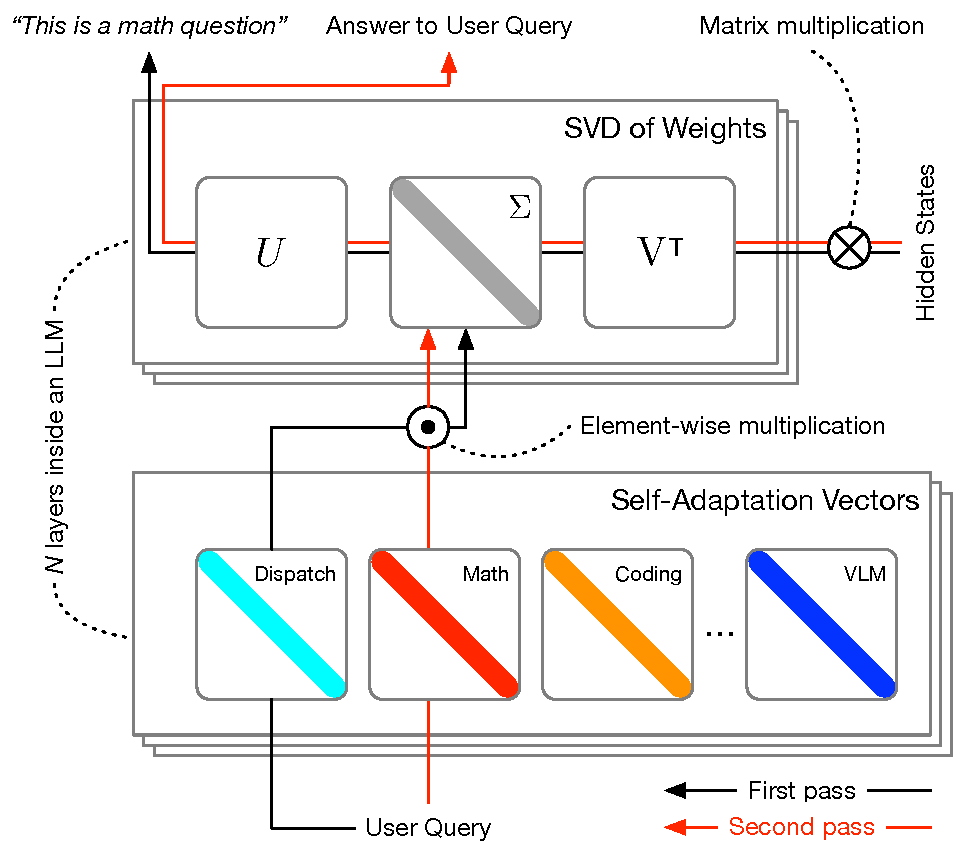
\includegraphics[width=0.6\textwidth,height=0.4\textwidth,keepaspectratio]{images/cover.pdf}
    \end{center}
  \vspace{-4mm}
  \caption{\textbf{Overview of \implname.} In the training phase, we tune the scales of the singular values of the weight matrices to generate a set of ``expert'' vectors, each of which specializes in one type of tasks. In the inference phase, a two-pass process is adopted where the first applies the task-specific expert and the second generates the answer.}
  \label{fig:cover}
  \vspace{-4mm}
\end{wrapfigure}

Self-adaptive large language models (LLMs) would represent a significant advancement in artificial intelligence, providing a framework where models can adjust to varied tasks and dynamic contexts in real time.
While compositionality and scalability are crucial for effective adaptation, current LLM training methodologies fall short of achieving both these properties simultaneously.
Our research aims to present a pioneering solution to realize this vision and address these gaps.

Traditionally, LLM post-training has sought to optimize a model for a wide range of capabilities in a single, extensive training session.
While this ``one-shot’’ fine-tuning framework is ideal from a simplicity perspective, it is also difficult to achieve in practice.
For instance, post-training is still highly resource-intensive, leading to significant computational costs and training times.
Additionally, there tends to be notable performance trade-offs when introducing additional breadth to the data, making it challenging to overcome overfitting and task interference at the same time.

In contrast, self-adaptive models offer a more flexible and efficient approach.
Rather than attempting to train an LLM for all tasks in one step, expert modules can be developed offline and augmented to the base LLM on-demand~\citep{kang2024self}.
This allows the model to dynamically modify its behavior based on the task at hand, without the need for constant re-tuning.
In addition to the benefit of having independent components, this modularity also supports continual learning, enabling the model to add new skills over time without catastrophic forgetting.
Moreover, self-adaptive LLMs mirror a well-established principle in neuroscience and computational biology, where the brain activates specific regions depending on the task at hand~\citep{loose2017switch} and dynamically reconfigures its functional networks in response to changing task demands~\citep{davison2015brain}.

In principle, the first step toward achieving self-adaptive LLMs can be realized through the development of specialized expert modules, each fine-tuned~\citep{kaplan2020scaling} via techniques such as low-rank adaptation (LoRA)~\citep{hu2021lora}.
These expert modules can then be dynamically composed at runtime based on the task demands, a process that can be efficiently managed through Mixture of Experts (MoE)-like systems~\citep{ICML2024_MoE}.
However, several challenges need to be addressed to make this approach both scalable and compositional.
First, fine-tuning LLMs to create multiple expert modules significantly increases the number of parameters that need to be trained.
In practice, even with parameter-efficient methods like LoRA, the cumulative size of these modules can quickly escalate, leading to increased storage and computational demands.
Second, these expert modules are often prone to overfitting, a phenomenon especially prevalent when training on smaller datasets or narrow task domains.
Third, the flexible composition of these expert modules also presents largely unresolved challenges currently posing as open research problems. 

To overcome these limitations, we first propose \svdname (\svdacro), a novel parameter-efficient fine-tuning (PEFT) method to obtain effective building blocks for self-adaptation.
\svdacro works by extracting and tuning only the singular values within the model's weight matrices.
By focusing on this principled parameterization, our approach mitigates the risk of overfitting, drastically reduces computational demands, and allows for inherent compositionality.
We show these properties enable us to cheaply obtain a set of effective domain-specific ``expert’’ vectors by training on narrow datasets with RL, directly optimizing task performance on individual topics.

We then introduce our full \implname framework to empower LLMs through the underlying principles of self-adaptation.
Given a prompt from an unknown task, \implname entails a two-pass inference mechanism which we illustrate in Figure~\ref{fig:cover}.
During the first pass, \implname executes the model and observes its test-time behavior, gathering the relevant information to understand the necessary skills to tackle the current problem.
During the second pass, our framework uses this information to combine the available expert vectors and provide a new modification to the base weights of the LLM specifically tailored to its test-time conditions. 
We design three different adaptation strategies that can be used within \implname, which we show provide monotonic performance benefits with increasing access to the test-time conditions.

We evaluate \svdacro and the full \implname framework through extensive experiments across a diverse range of LLMs and tasks.
First, when trained on domain-specific datasets, we show that \svdacro consistently outperforms traditional strategies for efficient fine-tuning such as LoRA, and at the same time, with orders of magnitudes fewer parameters.
Then we show that \implname is able to push performance far further, effectively adapting the weights of the base model even in entirely out-of-distribution applications such as visual question answering.
Finally, we analyze the properties of our new framework, validating that it provides increasing benefits with additional access to its current test-time conditions and even allow for recycling pre-trained \svdacro experts across model architectures.
In summary, our key technical contributions are the following: 
\begin{itemize}
\item The development of \implname as a pivotal self-adaptation framework for LLMs, providing a universal blueprint to dynamically adapt the behavior of LLMs from a growing set of pre-trained skills.
\item The introduction of \svdacro, a novel PEFT method trainable with RL on small datasets, producing compact expert vectors with inherent compositionality, all key properties necessary for our scalable self-adaptation framework.
\item The implementation of three adaptation strategies within \implname, effectively dispatching \svdacro-trained experts with properties designed to cope with different requirements and deployment scenarios.
\end{itemize}

\section{Related works}
\label{sec:relatedworks}

\textbf{Self-adaptive LLMs} We define self-adaptive LLMs as a group of LLMs or a standalone LLM that can evaluate and modify its behavior in response to changes in its operating environment or internal state, without external intervention.
This adaptation can be explored from two perspectives: a macroview, where multiple LLMs collaborate and/or compete, and a microview, where internal adaptations allow a single LLM to specialize in different tasks.

\textit{Macroview:} From this perspective, the system directs queries to LLMs with domain specific expertise, prioritizing outputs from expert models, thereby achieving higher accuracy and task-specific optimization.
Such task-specific ensembles can be realized through various mechanisms: multiple LLMs playing distinct roles and coordinate toward a shared goal~\citep{zhuge2023mindstorms}, engaging in mutual listening and debate~\citep{du2023improving}, or using meticulously crafted prompt constructions~\citep{zhang2024proagent} to integrate knowledge library and skill planning.
Naturally, the improvement in the specialization and adaptive capabilities of individual LLMs in the ensemble enhances the collective performance.
Thus, in this paper, we focus on the microview of self-adaptive LLMs.

\textit{Microview:} MoE in LLMs plays a critical role in this perspective~\citep{ICML2024_MoE}.
In MoE systems, inputs are dynamically routed to a subset of specialized modules or layers (e.g., MLPs) containing domain-specific knowledge~\citep{rajbhandari2022deepspeed,fedus2022switch}.
To reduce inference time, researchers introduce sparsely activated MoE where only a subset of the experts are selected per token~\cite{jiang2024mixtral,qwen_team_2024}.
While it is possible to view \implname loosely as a type of MoE, there are two major differences.
In the aforementioned systems, self-adaptation is achieved through token-level routing, whereas \implname employs a sample-level module selection strategy.
The second difference lies in the construction of expert modules.
In traditional MoE systems, expert modules are either trained from scratch~\citep{fedus2022switch,jiang2024mixtral} or dense models (e.g., upcycling)~\citep{qwen_team_2024,zhu2024llama}, without an auxiliary loss to ensure module specialization.
In contrast, \implname specifically trains expert vectors with RL to acquire domain specific-knowledge, making them true experts.

\textbf{Low-rank adaptation}
PEFT methods such as LoRA~\citep{hu2021lora} works by freezing the original model's parameters and introducing small trainable low-rank matrices for task-specific updates.
It significantly lowers the computational and memory costs while providing performance comparable to full fine-tuning.
Inspired by LoRA's design, various modifications have been proposed~\citep{zhang2023adalora,kopiczko2023vera,liu2024dora,balazy2024lora,huggingface2023svdtraining}.
\implname does not rely on low-rank matrices, and instead scales the singular vectors of the original parameter matrix that span the full rank space.

\textbf{SVD for LLM Fine-tuning}
SVD is increasingly being used as an inductive bias for PEFT in LLMs.
For example, \citet{wang2024milora} decompose a weight matrix and use the minor singular components, associated with noisy or long-tail information, to initialize low-rank matrices for LoRA fine-tuning.
In a similar vein, SVD is employed to approximate an original weight matrix with the top $r$ singular vectors, corresponding to the highest singular values.
A small trainable matrix is then introduced on top of the truncated singular value matrix to adjust the magnitude and orientations within this top-$r$ subspace~\citep{balazy2024lora,huggingface2023svdtraining}.
However, the drawback of this approach is that retaining only the top singular components can result in the loss of important information, particularly when the singular values distribution is less skewed.
The work most similar to ours is a concurrent effort by \citet{lingam2024svft}, where they introduce various sparsification methods that utilize the SVD of the weights.
However, it is not for self-adaptive LLMs and does not use RL to enhance learning efficiency.
\section{Methods}
\label{sec:methods}

\subsection{Preliminaries}

\textbf{Singular value decomposition (SVD)} offers a fundamental view of matrix multiplications.
In the context of neural networks, each weight matrix $W \in \mathbb{R}^{n \times m}$ can be decomposed into three components $W = U \Sigma V^\intercal$, yielding semi-orthogonal matrices $U \in \mathbb{R}^{m \times r}$ and $V \in \mathbb{R}^{n \times r}$ together with an ordered vector of $r$ singular values (in descending order) arranged in the diagonal matrix $\Sigma \in \mathbb{R}^{r \times r}$.
The linear operation defined by applying $W$ onto $x$, can be then decomposed into a sum of independent terms, derived from mapping each column $v_i$ from $V$ into the corresponding column $u_i$ from $U$ as $y=\sum_{i=1}^r \sigma_i u_i v_i^\intercal x$.
Hence, each singular component represented by the rank-1 matrix $u_i v_i^\intercal$ independently processes the input, providing an orthogonal contribution to the layer's outputs, with the singular values $\sigma_i$ modulating the degree of the contributions.

\textbf{Cross-entropy method (CEM)} is a Monte Carlo method for importance sampling and optimization~\citep{rubinstein2004cross}.
The method is based on the concept of minimizing the KL divergence between two probability distributions $D_\mathrm{KL}(P\|Q)$, where $P$ is the target distribution and $Q$ is a maintained distribution. 
At its core, CEM repeatedly generates a set of samples from $Q$, evaluates these samples with a performance function, and then updates the distribution $Q$ with the characteristics of the elite samples that have performed best. In the standard setup employed in most applications, $Q$ is set to a diagonal multivariate Gaussian, reducing the problem to simply estimating the empirical mean and standard deviation of the latest elites until a stopping criterion is met.
We illustrate a complete CEM step in the Python pseudocode below.

\begin{figure}[!h]
    \centering
    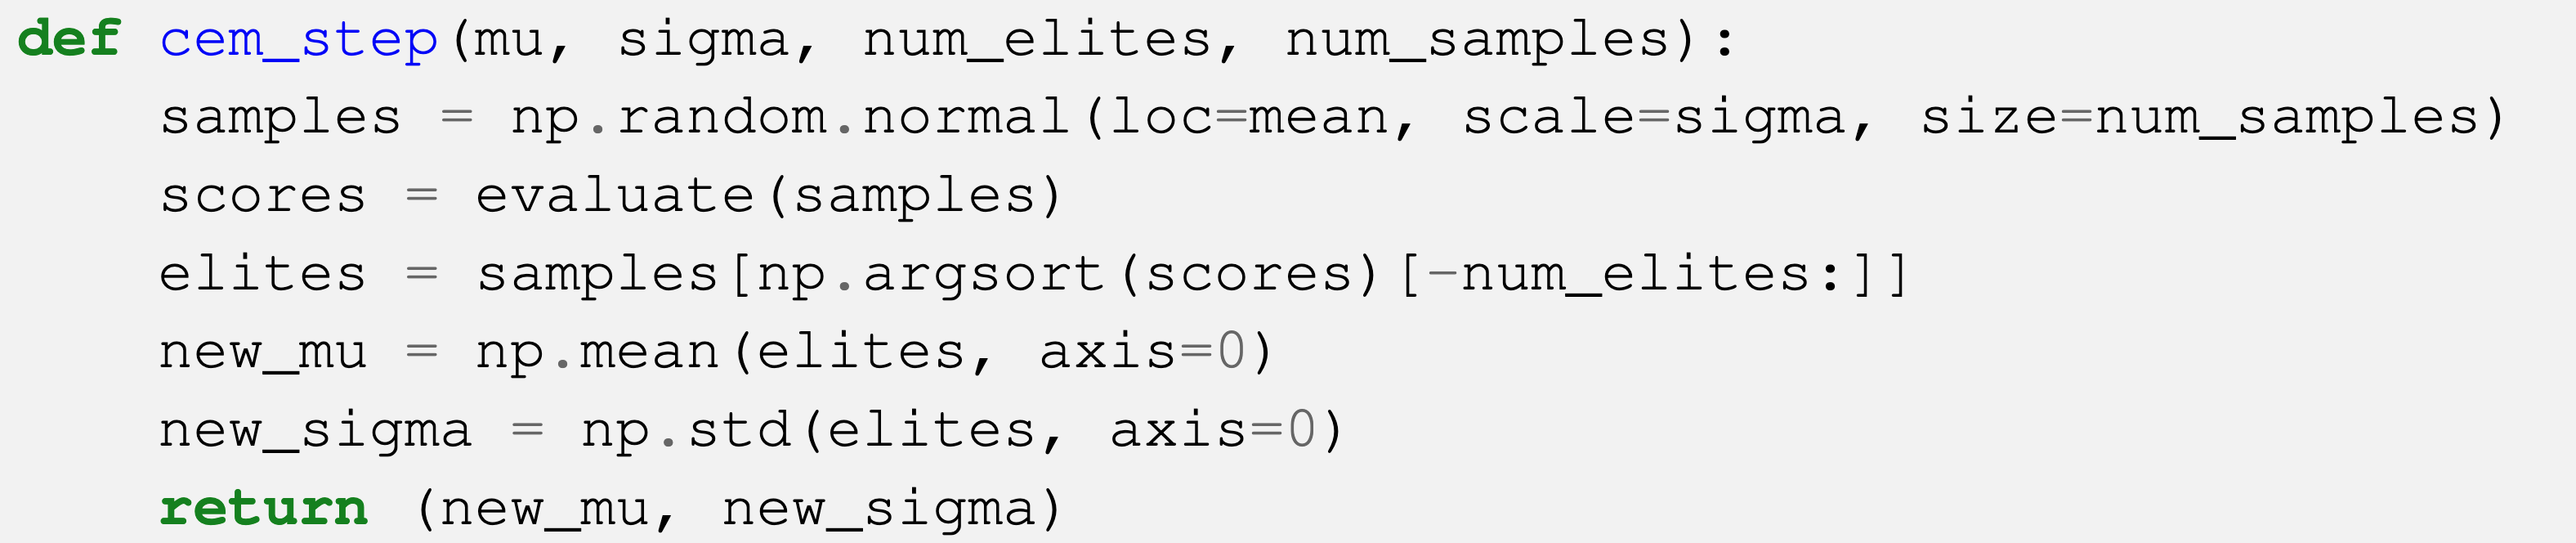
\includegraphics[width=\textwidth]{images/cem_code.png}
    \label{fig:cem_code}
\vspace{-5mm}
\end{figure}

\subsection{\textsc{\implname}}
\label{sec:transformer^2}

The construction of \implname comprises two main steps, for which we provide an illustrative overview in Figure~\ref{fig:method_overview}.
First, we introduce \svdname (\svdacro), a method to learn with RL compact and \textit{compositional} expert vectors based on the SVD of the base model's weights.
Then, we describe three different adaptation strategies within \implname, inspired by three orthogonal principles, which adaptively combine the \svdacro-trained expert vectors during inference.
We motivate how the properties of \svdacro are highly complementary to our adaptation strategies, making \implname an effective and scalable framework for the design of new self-adaptive LLMs.

\begin{figure}[!h]
    \centering
    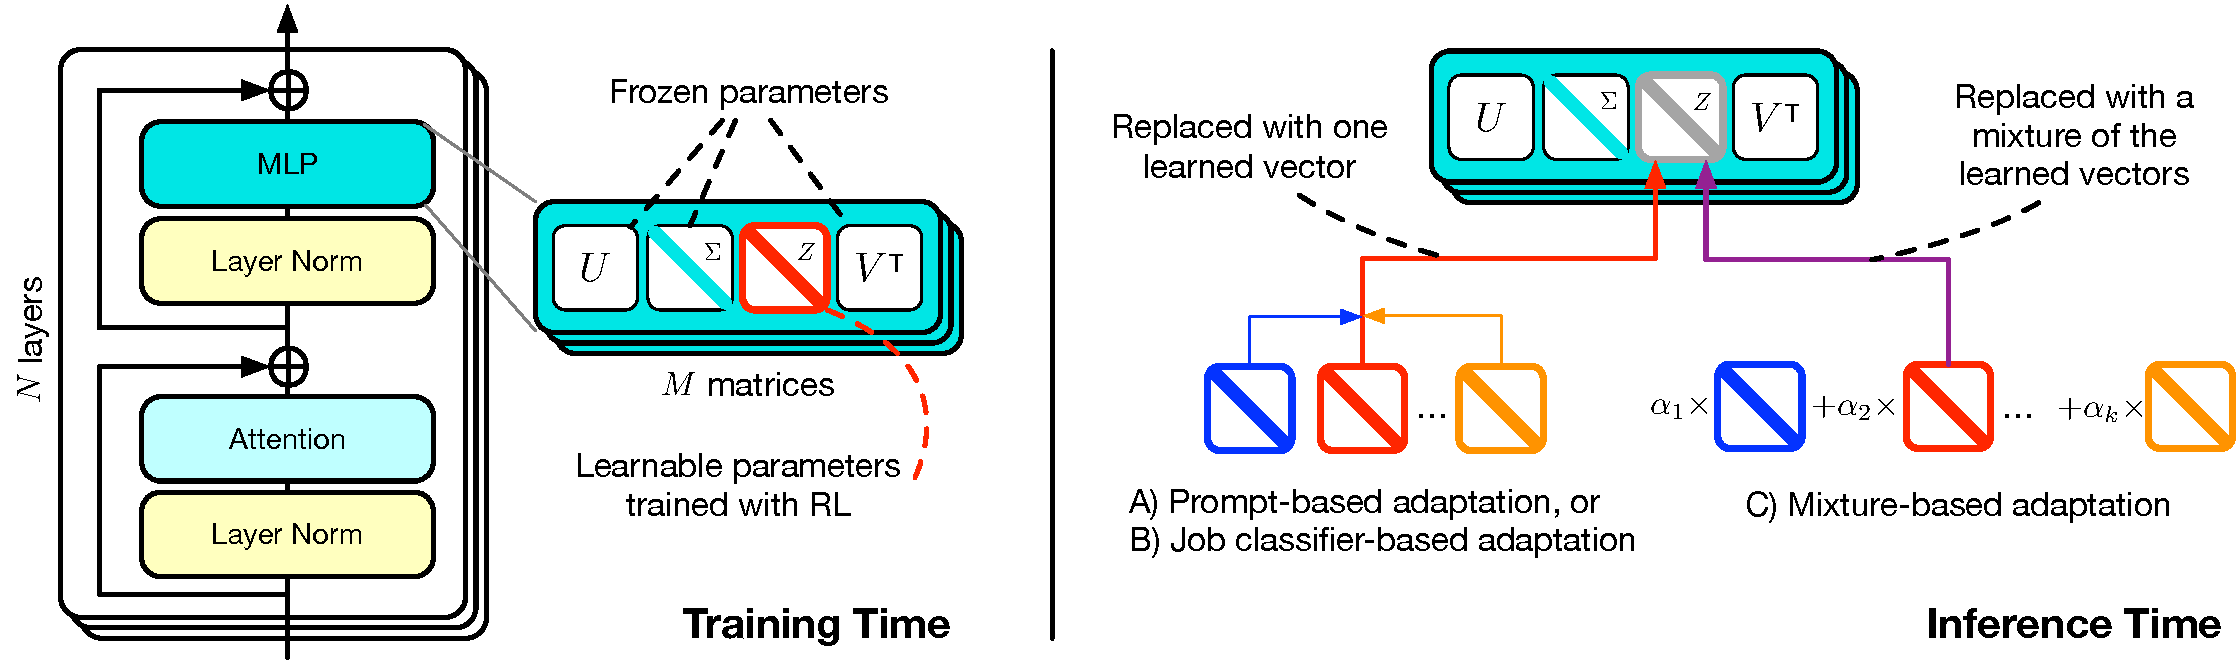
\includegraphics[width=\textwidth]{images/method_overview.pdf}
    % \vspace{-4mm}
    \caption{\textbf{Method overview.}
    Left) At training time, we employ \svdacro and RL to learn the ``expert'' vectors $z$'s that scale the singular values of the weight matrices.
    Right) At inference time, we propose three distinct methods to adaptively select/combine the learned expert vectors.
    }
    % \vspace{-2mm}
    \label{fig:method_overview}
\end{figure}


\textbf{Singular value fine-tuning}\label{sec:svf} is a key building block in \implname.
It offers an extremely efficient parameterization for fine-tuning and provides inherent compositionality for adaptation.
Conventional fine-tuning techniques often aim to augment pre-trained models with new capabilities by modifying their weight matrices.
However, in large-scale transformers,  these weights are already rich repositories of abstracted knowledge, thanks to the breadth of the pre-training data and expansive architectural design.
In fact, as evidenced in much of the prior literature, the requisite capabilities for solving many downstream tasks appear to already exist within these pre-trained models~\citep{sharma2023truth}.
Therefore, instead of seeking to add new features, an efficient fine-tuning approach should focus on making these latent capabilities more expressible. Motivated by these considerations, for any weight matrix $W$, \svdacro learns a simple vector $z\in \mathbb{R}^r$ that provides targeted modifications to each singular component of  $W$ independently, yielding a new weight matrix $W^\prime=U \Sigma^\prime V^\intercal$, where $\Sigma^\prime=\Sigma \otimes\text{diag}(z)$.
This essential parameterization enjoys several benefits:

\textit{Negligible parameters:} Learning only a vector $z$ for each weight matrix allows for very efficient fine-tuning with orders of magnitudes fewer optimized parameters even when compared to prior approaches specifically designed for efficiency. 
For example, the widely popular LoRA approach requires $(m + n) \times r^\prime$ learnable parameters per weight matrix, where $r^\prime$ is a hyper-parameter that generally needs to be set large enough for expressivity. While recent extensions, such LoRA-XS~\citep{balazy2024lora}, try to push efficiency even further, they often introduce limiting assumptions that curb applicability in several practical scenarios (see examples in Appendix~\ref{app:sec:pca}). 
In contrast, while \svdacro only needs $r=\min(m, n)$ parameters, we show it empirically does not display the same shortcomings thanks to working on a highly-meaning space provided by the latent expressiveness compressed in the weights of modern LLMs.
\svdacro's scaling only the singular values may seem to lead to limited expressiveness, we wish to point out that the ability to affect the weight matrix in a full-rank manner technically provides more information than low-rank approaches.

\textit{High compositionality:} Decomposing the weights in independent singular components makes the learned $z$ vectors highly composable and interpretable, opening numerous possibilities for adaptation via algebraic manipulations.
Instead, LoRA-based methods inherently lack these properties. 
For instance, even if two LoRAs learned on the same task were to learn exactly the same adjustments for each $W$, directly interpolating between their compressed $A$ and $B$ matrices is unlikely to preserve any of their original behavior, given the countless number of equivalent parameter permutations they might have converged to.

\textit{Principled regularization:} Exclusively modifying the magnitude of pre-existing singular components provides a principled and effective form of regularization.
In practice, this property enables us to fine-tune for arbitrary downstream tasks with only hundreds of data points without the risk of severe collapse or overfitting.

\textbf{End-to-end optimization with RL.} We train a set of \svdacro vectors $\theta_z = \{z_1, \cdots, z_{N \times M}\}$ to fine-tune an arbitrary language model $\pi_{\theta_W}$ parameterized by $\theta_{W}$ with RL, optimizing directly for task performance.
Here, $\theta_{W}=\{ W_1, \cdots, W_{N \times M} \}$ is the set of weight matrices, where $N$ is the number of layers and $M$ is the number of weight matrices to fine-tune per layer.
We use the seminal REINFORCE algorithm~\citep{williams1992simple} and label each generated answer $y_i$ (for the prompt $x_i\in D$) with a unitary reward based on its correctness $r\in \{-1, 1\}$.
Inspired by related applications of RL for optimizing LLMs~\citep{ouyang2022training}, we regularize the REINFORCE objective by adding a KL penalty for deviating from the original model's behavior, weighted by a small coefficient $\lambda \in \mathbb{R^+}$. Thus, our final objective function can be written as:
\begin{equation}
    J(\theta_z) = \E \left[\log\left(\pi_{\theta_{W^\prime}}(\hat{y}_i \mid x_i)\right)r(\hat{y}_i, y_i)\right] - \lambda D_\mathrm{KL}(\pi_{\theta_{W^\prime}} \| \pi_{\theta_{W}}),
\label{eqn:sec3:reinforce}
\end{equation}
where we use $\pi_{\theta_{W^\prime}}$ to denote the resulting language model after substituting the original weight matrices $W$ with $W^\prime$.
While RL is generally considered less stable than next-token prediction objectives, we find the regularization properties of SVF avoid many of the failure modes of prior less-constrained parameterizations (see Section~\ref{app:sec:ablation_studies}).
Thus, combining these complementary components effectively enables us to avoid relying on expensive fine-tuning procedures with large hand-designed datasets as proxies, and directly maximize task performance end-to-end.

In general, \svdacro with RL puts lower requirement on the dataset it trains on.
For example, LoRA fine-tuning requires ``explaining texts'' to perform next token predictions, which puts a higher requirement on the dataset (e.g., imagine LoRA fine-tuning on a GSM8K dataset where no reasoning text but only the final number is provided).
This benefit allows \svdacro to be more general and effective.
One possible caveat \svdacro can face is the sparse rewards caused by a weak base model, which we discuss this further in Section~\ref{sec:conclusion}.

\textbf{Self-adaptation} is a critical mechanism in nature that has established itself as a core guiding principle in modern system design \citep{7302492}. Our initial efforts toward self-adaptive foundation models focus on the inference stage of LLMs, where we devise a simple two-pass adaptation strategy that combines $K$ sets of base ``expert'' vectors $z^{1:K}$ trained with \svdacro to provide different kinds of capabilities (e.g., coding, math, etc).
The mapping between a capability and the dataset we train on can be acquired in the dataset's meta data.
In the first inference pass, given a task or an individual input prompt, \implname executes the model and observes its test-time behavior to derive a new $z'$ vector tailored to its test-time conditions. 
This adapted $z'$ is then used in the second inference pass to provide an actual response with the newly adapted weights.
The interaction between \svdacro-trained expert vectors and the adaptation strategies ensures seamless integration, where expert vectors provide modular capabilities, and the adaptation strategies dynamically determine and compose the most suitable combination to address the input task.
In this first work, we propose three simple approaches to produce the vector $z'$ during the first inference pass, implementing self-adaption with distinct methods and requirements. Below, we provide an outline of each method and refer to Appendix~\ref{app:sec:implementation} for additional implementation details.


\textit{A) Prompt engineering:}
Our most basic approach involves constructing a new ``adaptation'' prompt which we use to directly \textit{ask} the LLM to categorize the input prompt.
Based on its response, we then extract one category out of the set of domain topics used to pre-train each \svdacro expert and, thus, we select the corresponding $z'$ directly from $z^{1:K}$.
In our adaptation prompt, we also explicitly provide the option for a generic ``others'' category, allowing the model to use its base weights in case no expert provides appropriate capabilities. We show the format used to construct the adaptation prompt in Figure~\ref{fig:sys_prompt}.

\begin{wrapfigure}{r}{0.45\textwidth}
\vspace{-8mm}
\begin{center}
    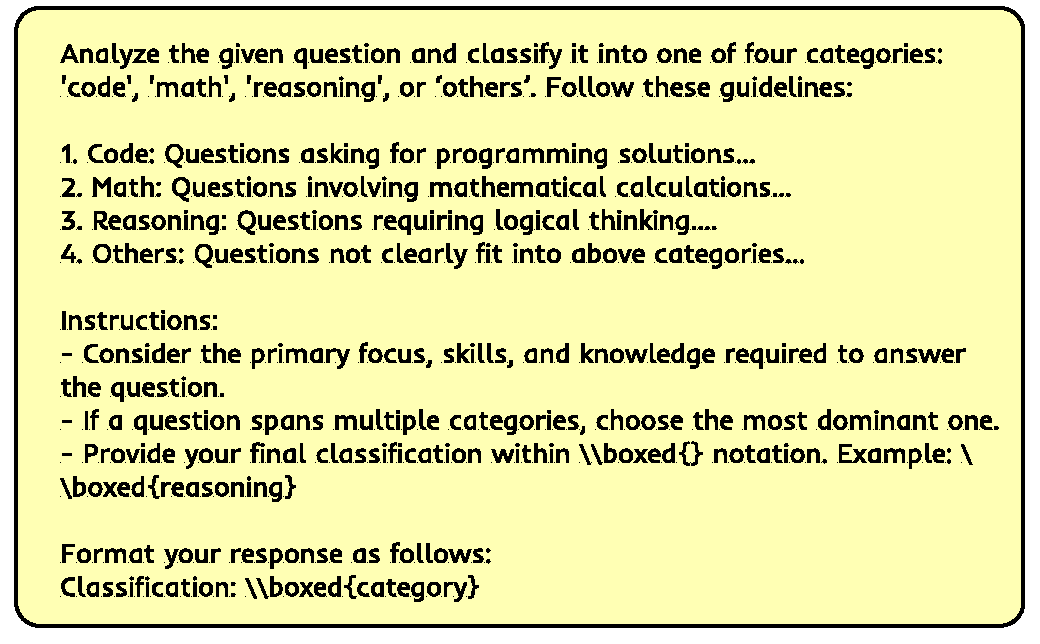
\includegraphics[width=0.45\textwidth]{images/visualization/system_prompt.pdf}
  \end{center}
  \vspace{-5.5mm} 
  \caption{\textbf{Prompt based adaptation.} Self-adaptation prompt used by \implname to classify the task prompt into pre-defined categories.}
  \label{fig:sys_prompt}
  \vspace{-4mm}
\end{wrapfigure}

\textit{B) Classification expert:} 
A direct extension of the prompt engineering approach comes from using a specialized system to handle task identification.
Following the principles of self-adaptation, we apply \svdacro to fine-tune the base LLM itself to handle this task.
In particular, we collect a dataset $D = \{(x_{1,1}, 1), \cdots, (x_{i,k}, k), \cdots \}$ from the $K$ \svdacro training tasks, where $x_{i,k}$ is the $i$-th example from the $k$-th expert task.
Each tuple $(x_{i,k}, k)$ then forms an example to pre-train an additional job classification expert $z^c$ learned in the same fashion as the others.
During the first inference pass, we simply load $z^c$, intending to improve the inherent task classification capabilities of the base model to select a more appropriate $z'$ to handle the input prompt. 

\textit{C) Few-shot adaptation:} Our third approach leverages additional task information by assuming extended access to its test-time conditions beyond individual prompts. 
Our approach is inspired by popular few-shot prompting techniques, which have been shown to provide consistent performance improvements and even allow LLMs to ``in-context'' learn tasks that were entirely unseen prior to inference~\citep{brown2020language}.
For each optimized $W$, our approach entails producing an entirely new $z^\prime=\sum^{K}_{k=1} \alpha_k z_k$ by linearly interpolating between the $K$ learned \svdacro vectors, each weighted by the coefficients $\alpha_k$.
We employ CEM to search over the possible values of each $\alpha_k$ based on the performance on a set of ``few-shot prompts'', which are specifically held out from the rest of the test prompts and used to evaluate CEM's population samples. 
In the case of multiple population samples obtaining the same score on these held-out prompts, we break ties by favoring the one with the highest average log-likelihood across its own generated correct answers.
Crucially, we only need to perform this process once for each target task, avoiding the need to increase the length of each question prompt, a relevant downside of traditional few-shot prompting. We refer to Section~\ref{app:sec:fewshot}, for additional details and an extended discussion of this final approach. 

\vspace{-2mm}
\section{Experiments}
\label{sec:experiments}

\vspace{-2mm}

We extensively evaluate \implname on multiple tasks and models with the purpose of:
(1) assessing the efficiency and effectiveness of \svdacro;
(2) demonstrating self-adaptiveness through the three proposed adaptation strategies;
(3) conducting in-depth analysis and ablation studies aimed at understanding and interpreting the properties of our new framework.

\vspace{-2mm}
\subsection{Experimental setups}
\vspace{-1mm}

To validate the generality of \implname we consider three pre-trained LLMs ranging across different model families and architecture sizes: \llama, \mistral, and \llamaXL.
For each model, we obtain three sets of \svdacro-trained $z$ vectors to maximize performance for GSM8K~\citep{cobbe2021training},  MBPP-pro~\citep{austin2021program}, and ARC-Easy~\citep{clark2018think}, respectively.
Additionally, we also train a set of $z$ vectors for \llama, when applied as the language backbone for TextVQA~\citep{singh2019towards}, in order to assess \svdacro's applicability to the vision-language modeling (VLM) domain.
We provide \svdacro's main learning curves on each of these tasks in Figure~\ref{fig:learning_curves}. 
Finally, we evaluate the full \implname adaptation framework on four unseen tasks: MATH~\citep{hendrycks2021measuring}, Humaneval~\citep{chen2021evaluating}, ARC-Challenge~\citep{clark2018think}, and OKVQA~\citep{marino2019ok}. In all our adaptation experiments, we only consider experts obtained in the pure-language settings, assessing its test-time applicability even for the distinctive vision domain. 
Please refer to the Appendix~\ref{app:sec:implementation} for additional details and a summary of the hyper-parameters used in the experiments.

\begin{figure}[!t]
    \centering
    % \vspace{-4mm}
    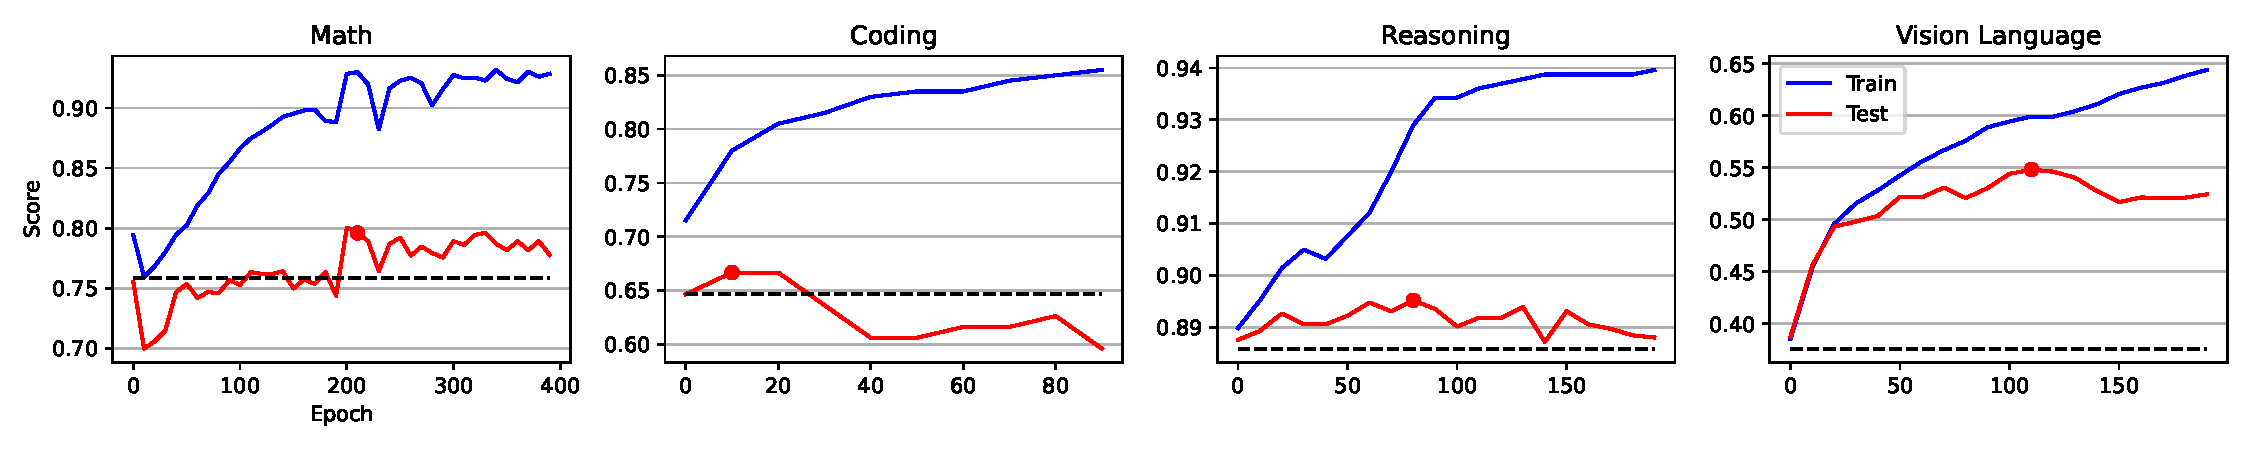
\includegraphics[width=0.95\textwidth]{images/learning_curves_new.pdf}
    \vspace{-4mm}
    \caption{\textbf{\svdacro learning curves.} The dashed lines indicate the performance of \llama on the test split of each task. SVF effectively fine-tunes to surpass the base performance. While we use the best validation score to select our checkpoint for evaluation (marked by red dots), we present the entire training curve without early stopping to demonstrate \svdacro's learning capabilities. Tasks with only hundreds of training samples like Coding and Reasoning were stopped early. In our experiments, we update the parameters at the end of each epoch.}
    \vspace{-6mm}
    \label{fig:learning_curves}
\end{figure}


\subsection{Experimental results}

% \begin{table}[!t]
% \centering

% \caption{\textbf{LLM Fine-tuning Results.} LLM performance on the test splits.}

% \small
% \begin{tabular}{llll}
% \toprule

% \textbf{Method} & \textbf{GSM8K} & \textbf{MBPP-Pro} & \textbf{ARC-Easy} \\

% \midrule
% \llama & {\normalsize 75.89 {\footnotesize (\grey{1.00})}} & {\normalsize 64.65 {\footnotesize (\grey{1.00})}} & {\normalsize 88.59 {\footnotesize (\grey{1.00})}} \\
% \quad + LoRA & {\normalsize 70.58 {\footnotesize (\red{0.93})}} & \textbf{{\normalsize 67.68 {\footnotesize (\green{1.05})}}} & {\normalsize 88.97 {\footnotesize (\grey{1.00})}} \\
% \quad + SVF (Ours) & \textbf{{\normalsize 79.15 {\footnotesize (\green{1.04})}}} & {\normalsize 66.67 {\footnotesize (\green{1.03})}} & \textbf{{\normalsize 89.56 {\footnotesize (\green{1.01})}}} \\

% \midrule
% \mistral & {\normalsize 42.83 {\footnotesize (\grey{1.00})}} & {\normalsize 49.50 {\footnotesize (\grey{1.00})}} & {\normalsize 49.50 {\footnotesize (\grey{1.00})}} \\
% \quad + LoRA & {\normalsize 36.09 {\footnotesize (\red{0.84})}} & {\normalsize 47.47 {\footnotesize (\red{0.96})}} & {\normalsize 47.47 {\footnotesize (\red{0.96})}} \\
% \quad + SVF (Ours) & \textbf{{\normalsize 49.74 {\footnotesize (\green{1.16})}}} & \textbf{{\normalsize 51.52 {\footnotesize (\green{1.04})}}} & \textbf{{\normalsize 85.14 {\footnotesize (\green{1.72})}}} \\

% \midrule
% \llamaXL & {\normalsize 85.29 {\footnotesize (\grey{1.00})}} & \textbf{{\normalsize 80.81 {\footnotesize (\grey{1.00})}}} & \textbf{{\normalsize 89.10 {\footnotesize (\grey{1.00})}}} \\
% \quad + SVF (Ours) & \textbf{{\normalsize 88.32 {\footnotesize (\green{1.04})}}} & \textbf{{\normalsize 80.81 {\footnotesize (\grey{1.00})}}} & {\normalsize 88.47 {\footnotesize (\red{0.99})}} \\

% \bottomrule
% \end{tabular}

% \label{tab:res:svf_train_tasks}
% \end{table}

% \begin{figure}[!t]
%     \centering
%     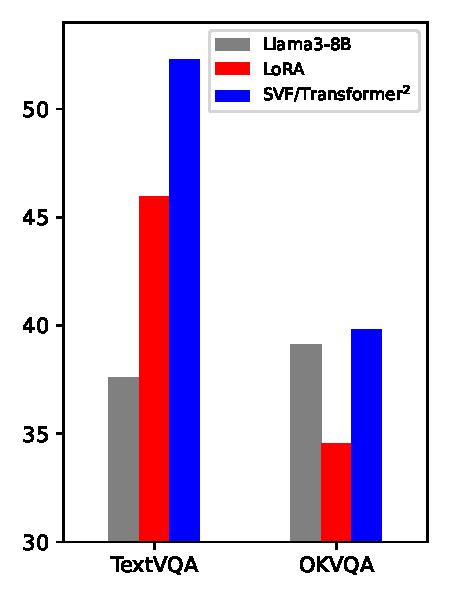
\includegraphics[width=\textwidth]{images/vlm_barplot.pdf}
%     % \vspace{-8mm}
%     \caption{\textbf{VLM Results.}
%     }
%     % \vspace{-4mm}
%     \label{fig:vlm_results}
% \end{figure}



\begin{figure}[!b]
    \vspace{-4mm}
    \centering

    % Left side: Table
    \begin{minipage}{0.75\linewidth}
        \centering
        \captionof{table}{\textbf{Fine-tuning results.} LLM performance on the test splits of math, coding and reasoning. Normalized scores are in the parentheses.}
        \vspace{-3.5mm}
        \small
        \begin{tabular}{llll}
            \toprule
            \textbf{Method} & \textbf{GSM8K} & \textbf{MBPP-Pro} & \textbf{ARC-Easy} \\
            \midrule
            \llama & {\normalsize 75.89 {\scriptsize (\grey{1.00})}} & {\normalsize 64.65 {\scriptsize (\grey{1.00})}} & {\normalsize 88.59 {\scriptsize (\grey{1.00})}} \\
            \quad + LoRA & {\normalsize 77.18 {\scriptsize (\green{1.02})}} & \textbf{{\normalsize 67.68 {\scriptsize (\green{1.05})}}} & {\normalsize 88.97 {\scriptsize (\grey{1.00})}} \\
            \quad + SVF (Ours) & \textbf{{\normalsize 79.15 {\scriptsize (\green{1.04})}}} & {\normalsize 66.67 {\scriptsize (\green{1.03})}} & \textbf{{\normalsize 89.56 {\scriptsize (\green{1.01})}}} \\
            \midrule
            \mistral & {\normalsize 42.83 {\scriptsize (\grey{1.00})}} & {\normalsize 49.50 {\scriptsize (\grey{1.00})}} & {\normalsize 81.65 {\scriptsize (\grey{1.00})}} \\
            \quad + LoRA & {\normalsize 44.66 {\scriptsize (\red{1.04})}} & {\normalsize 51.52 {\scriptsize (\green{1.04})}} & {\normalsize 81.19 {\scriptsize (\red{0.98})}} \\
            \quad + SVF (Ours) & \textbf{{\normalsize 49.74 {\scriptsize (\green{1.16})}}} & \textbf{{\normalsize 51.52 {\scriptsize (\green{1.04})}}} & \textbf{{\normalsize 85.14 {\scriptsize (\green{1.04})}}} \\
            \midrule            
            \llamaXL & {\normalsize 85.29 {\footnotesize (\grey{1.00})}} & \textbf{{\normalsize 80.81 {\footnotesize (\grey{1.00})}}} & \textbf{{\normalsize 89.10 {\footnotesize (\grey{1.00})}}} \\
            \quad + LoRA & {\normalsize 77.26 {\footnotesize (\red{0.91})}} & {\normalsize 68.69 {\footnotesize (\red{0.85})}} & {\normalsize 88.55 {\footnotesize (\red{0.99})}} \\
            \quad + SVF (Ours) & \textbf{{\normalsize 88.32 {\footnotesize (\green{1.04})}}} & \textbf{{\normalsize 80.81 {\footnotesize (\grey{1.00})}}} & {\normalsize 88.47 {\footnotesize (\red{0.99})}} \\
            \bottomrule                
        \end{tabular}
        \label{tab:res:svf_train_tasks}
    \end{minipage}
    \hfill
    % Right side: Figure
    \begin{minipage}{0.23\linewidth}
        \centering
        % \vspace{2mm}
        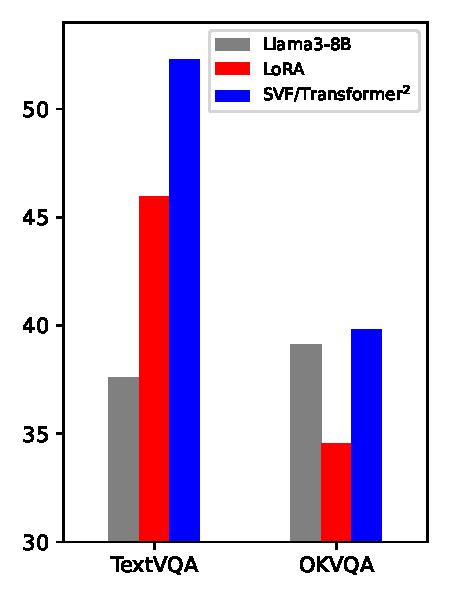
\includegraphics[width=\linewidth]{images/vlm_barplot.pdf}
        \vspace{-8mm}
        \captionof{figure}{\textbf{Results for the VLM domain.}}
        \label{fig:vlm_results}
    \end{minipage}

\end{figure}


\textbf{\svdacro performance}
We provide results after training on each considered task with the \llama, \mistral, and \llamaXL base models in Table~\ref{tab:res:svf_train_tasks}.
Remarkably, we find that \svdacro provides considerable and consistent performance gains across nearly all tasks and base models. Instead, LoRA experts yield smaller gains and even sporadic performance degradation.
(These LoRA experts are trained with next token prediction. While we also have LoRA experts trained with RL in Table~\ref{tab:res:ablation}, RL seems work less well with LoRA than with \svdacro.)
This observed trend extends also to the vision-language domain, as fine-tuning \textsc{Llama3-Llava-Next-8B} with \svdacro bolsters the base model's performance by over 39\% (see Figure~\ref{fig:vlm_results}).
To ensure a fair comparison, we provide extensive ablations to both our model and the LoRA baseline considering different architecture and optimization objectives in Appendix~ \ref{app:sec:ablation_studies}).
Due to its essential parameterization, we would like to note that training \svdacro requires considerably fewer resources, with less than 10\% of the training parameters of our LoRA implementation.

\textbf{Adaptation performance}
With the \svdacro trained $z$ vectors, we assess the self-adaptation capability of \implname on unseen tasks.
For a fair comparison with LoRA, we record the performance of this baseline using all checkpoints from the considered training tasks and report only its highest performance for each of the test tasks. 
As shown in Table~\ref{tab:res:svf_ada_tasks}, all of our \implname adaptation strategies demonstrate improvements across all tasks for \llama base models, and in at least two out of three tasks for both \mistral and \llamaXL.
In contrast, even the best training LoRAs only provide marginal improvements on the ARC-Challenge task and still significantly deteriorate performance on both MATH and Humaneval. 
This discrepancy suggests that LoRA's parameterization and optimization might be particularly sensitive to overfitting, especially when trained with the smaller GSM8K and MBPP-Pro datasets, the tasks that provide information most related to MATH and Humaneval.
In Figure~\ref{fig:vlm_results}, we find a similar dichotomy in the OKVQA task, with the performance of the base \textsc{Llama3-Llava-Next-8B} VLM only improving after applying \implname.
We note that also in this setting, \implname performs self-adaptation only from the expert vectors from GSM8K, MBPP-Pro, and ARC-Easy.
Thus, this result further underscores the high flexibility of self-adaptation, transferring knowledge compressed for tasks entirely based on language even for unrelated vision-based problems.

\begin{table}[!t]
\centering
\vspace{-2mm}
\caption{\textbf{Self-adaptation on unseen tasks.} Normalized scores are in the parentheses.}
% \vspace{-2mm}
\small
\begin{tabular}{llll}
\toprule
Method & MATH & Humaneval & ARC-Challenge \\

\midrule
\llama3 & {\normalsize 24.54 {\footnotesize (\grey{1.00})}} & {\normalsize 60.98 {\footnotesize (\grey{1.00})}} & {\normalsize 80.63 {\footnotesize (\grey{1.00})}} \\
\quad + LoRA & {\normalsize 21.68 {\footnotesize (\red{0.88})}} & {\normalsize 52.44 {\footnotesize (\red{0.86})}} & {\normalsize 81.06 {\footnotesize (\green{1.01})}} \\
\quad + \implname (Prompt) & {\normalsize 25.22 {\footnotesize (\green{1.03})}} & {\normalsize 61.59 {\footnotesize (\green{1.01})}} & {\normalsize 81.74 {\footnotesize (\green{1.01})}} \\
\quad + \implname (Cls-expert) & {\normalsize 25.18 {\footnotesize (\green{1.03})}} & {\normalsize 62.80 {\footnotesize (\green{1.03})}} & {\normalsize 81.37 {\footnotesize (\green{1.01})}} \\
\quad + \implname (Few-shot) & \textbf{{\normalsize 25.47 {\footnotesize (\green{1.04})}}} & \textbf{{\normalsize 62.99 {\footnotesize (\green{1.03})}}} & \textbf{{\normalsize 82.61 {\footnotesize (\green{1.02})}}} \\

\midrule
\mistral & {\normalsize 13.02 {\footnotesize (\grey{1.00})}} & {\normalsize 43.29 {\footnotesize (\grey{1.00})}} & {\normalsize 71.76 {\footnotesize (\grey{1.00})}} \\
\quad + LoRA & {\normalsize 11.18 {\footnotesize (\red{0.86})}} & {\normalsize 31.71 {\footnotesize (\red{0.73})}} & \textbf{{\normalsize 75.77 {\footnotesize (\green{1.06})}}} \\
\quad + \implname (Prompt) & {\normalsize 11.86 {\footnotesize (\red{0.91})}} & {\normalsize 43.90 {\footnotesize (\green{1.01})}} & {\normalsize 72.35 {\footnotesize (\green{1.01})}} \\
\quad + \implname (Cls-expert) & {\normalsize 11.60 {\footnotesize (\red{0.89})}} & {\normalsize 43.90 {\footnotesize (\green{1.01})}} & {\normalsize 74.83 {\footnotesize (\green{1.04})}} \\
\quad + \implname (Few-shot) & \textbf{{\normalsize 13.39 {\footnotesize (\green{1.03})}}} & \textbf{{\normalsize 47.40 {\footnotesize (\green{1.09})}}} & {\normalsize 75.47 {\footnotesize (\green{1.05})}} \\

\midrule
\llamaXL & \textbf{{\normalsize 40.64 {\footnotesize (\grey{1.00})}}} & {\normalsize 78.66 {\footnotesize (\grey{1.00})}} & {\normalsize 87.63 {\footnotesize (\grey{1.00})}} \\
\quad + LoRA & {\normalsize 25.40 {\footnotesize (\red{0.62})}} & {\normalsize 73.78 {\footnotesize (\red{0.94})}} & {\normalsize 83.70 {\footnotesize (\red{0.96})}} \\
\quad + \implname (Prompt) & {\normalsize 40.44 {\footnotesize (\grey{1.00})}} & \textbf{{\normalsize 79.88 {\footnotesize (\green{1.02})}}} & \textbf{{\normalsize 88.48 {\footnotesize (\green{1.01})}}} \\
\bottomrule

\end{tabular}

\label{tab:res:svf_ada_tasks}
\vspace{-6mm}
\end{table}



Comparing the three proposed adaptation strategies, we highlight a clear monotonic trend -- with more involved strategies and additional information about the test-time condition, self-adaptation appears to be increasingly effective.
In particular, \implname with few-shot self-adaptation is almost always the highest-scoring method, providing notable improvements across all tested settings except for \llamaXL@MATH, where we have only SVF-tuned half of the layers due to our limited GPU resources.
This trend shows that providing additional or different kinds of information seems to be highly beneficial to our framework, suggesting that \implname could provide foundation models with new means to continually improve performance when deployed in lifelong settings.

\begin{wraptable}{r}{0.35\textwidth}
\vspace{-6mm}
\centering
\caption{\textbf{Time cost of 2-pass inference in prompt adaptation strategy of \implname for the entire problem set.} 1st to 2nd pass inference time ratios are shown in parentheses.}
\label{tab:res:inference_time}
\vspace{-3.5mm}
\small
\resizebox{0.35\textwidth}{!}{
\begin{tabular}{lrr}
\toprule
\textbf{Task} & \textbf{1st (s)} & \textbf{2nd (s)} \\
\midrule
MATH         & 42.64    {\footnotesize (13\%)}             & 321.19                  \\
Humaneval    & 2.76   {\footnotesize (19\%)}                 & 14.28                   \\
ARC-Challenge & 13.40      {\footnotesize (47\%)}             & 28.51                   \\
\bottomrule
\end{tabular}
}
\vspace{-4mm}
\end{wraptable}

Table~\ref{tab:res:inference_time} reports the inference time required by the prompt adaptation strategy of \implname, with the time spent on solving the entire problem set presented separately for the 1st and 2nd passes.
Notice that the 2nd pass inference time is the time spent on solving the problems, and the 1st pass inference time is the time for self-adaptation, 1st to 2nd pass inference time ratios are in the parentheses.
While the additional inference pass might appear to double the overall runtime, it is important to note that inference time primarily depends on the number of tokens generated.
In our settings, it is $\mathcal{O}(n)$ where $n$ is the length of the input.
ARC-challenge's cost ratio is large because they are single choice problems and therefore the cost of the 2nd pass is also $\mathcal{O}(n)$.
In general settings, we think it is reasonable to assume this ratio to be closer to those of MATH and Humaneval.
For a detailed discussion on improving the efficiency of CEM few-shot adaptation methods, please see Appendix~\ref{app:sec:efficiency_improvements}

\subsection{Analysis}
\label{sec:analysis}

Lastly, we analyze and discuss the properties of our adaptation strategies for which we provide extensions and further discussion Appendix~\ref{app:sec:additional_exp}.

\textbf{Analysis 1: Job dispatching accuracy}
In Figure~\ref{fig:confusion_matrices} we provide the confusion matrices of our classification-based adaptation strategies. These results validate the effectiveness of both our classification-based adaptation strategies to match each prompt with experts trained in similar domains, as evidenced by the high values along the diagonals. 
Furthermore, the results from \llama and \mistral also show that using the classification expert consistently provides higher classification accuracy than vanilla prompt engineering.
While this difference could explain the higher performance of the relative self-adaptation strategy, we also note that domain similarity might not be the only metric relevant to identifying the best expert for each prompt or task.
To this end, we believe many further unexplored extensions could be explored in future work, using heuristics such as past expert performance or token-level analysis to further push our framework's scalability.

\begin{figure}[t]%[!b]
    \centering
    \vspace{-0.5mm}
    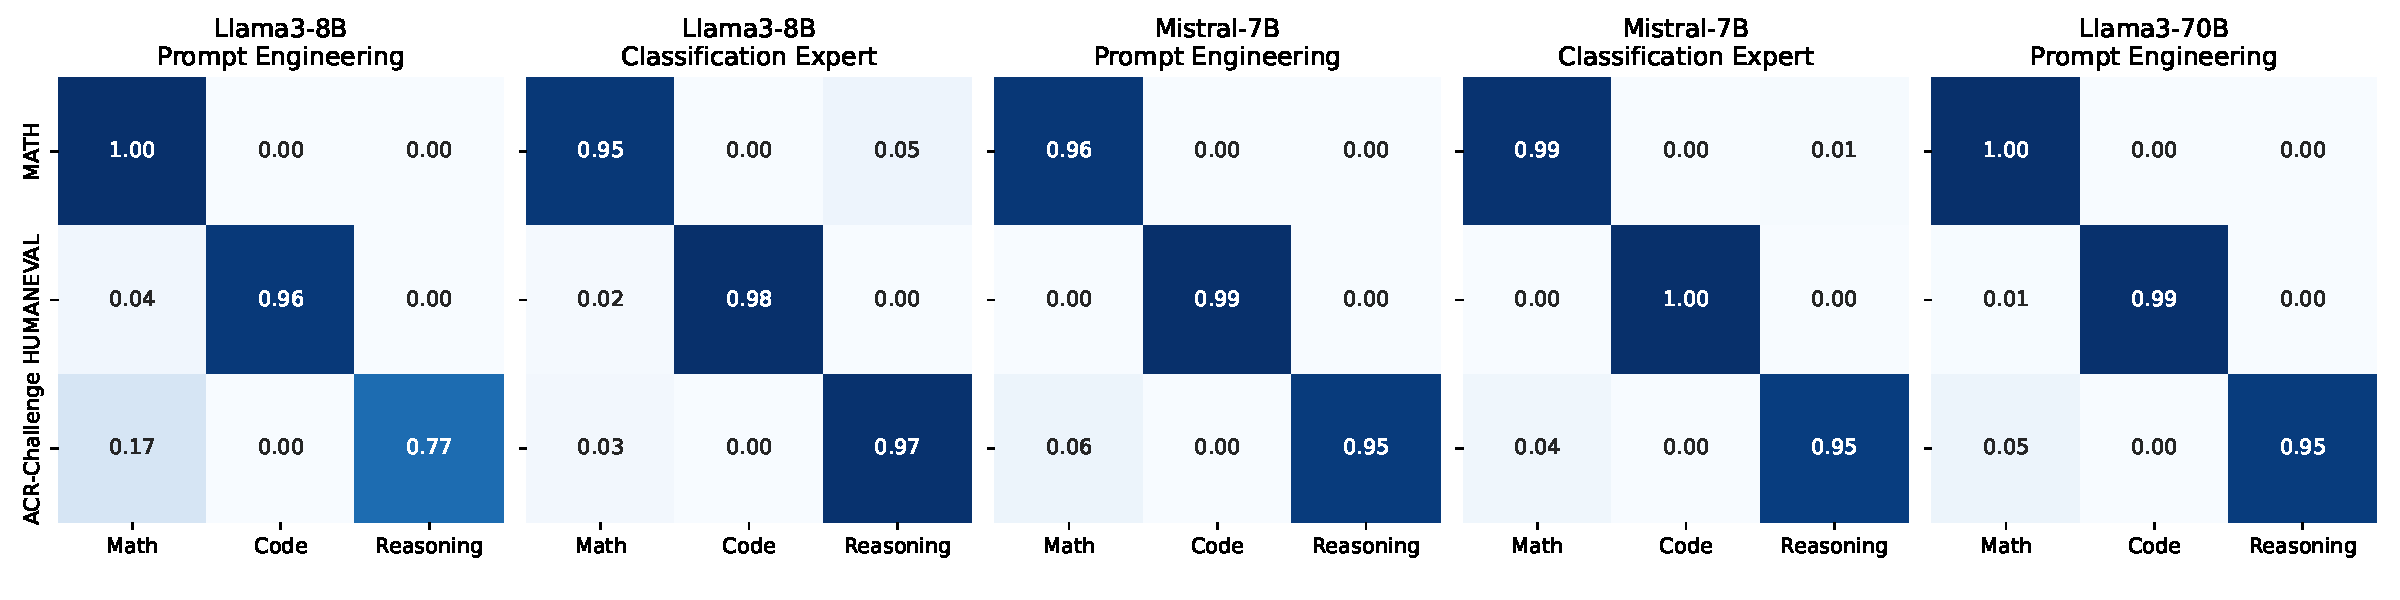
\includegraphics[width=0.9\textwidth]{images/confusion_matrices.pdf}
    \vspace{-4mm}
    \caption{\textbf{Confusion matrices.} These matrices display the classification percentages, where rows represent the task classes (ground truth) and columns indicate the predicted categories. Some samples are misclassified as ``Others,'' which is reflected in rows where the totals do not sum to one.
    }
    \vspace{-10mm}
    \label{fig:confusion_matrices}
\end{figure}

\textbf{Analysis 2: Training tasks adaptation contribution}
In Figure~\ref{fig:cem}, we show the normalized adaptive coefficients $a_k$ interpolating between our \svdacro vectors learned via CEM for \llama and \mistral across all the unseen downstream tasks. 
Intuitively, we find that the expert vectors from the training tasks sharing similar topics to the unseen ones are often the highest contributors to the produced adaptive weights. 
However, we observe that the MATH task appears as an interesting exception, as the $a_k$ for the expert obtained from GSM8K training is actually the lowest out of the three in both models.
We hypothesize this reflects the different nature of the mathematics competition problems from MATH as compared to the grade-school problems in GSM8K.
In fact, not only is the difficulty of the MATH questions far beyond GSM8K, but a large portion of its problems also hinges mainly on logical reasoning, for which a task like ARC might actually be more aligned.
Furthermore, we also note that the different $z$ vectors appear to contribute more uniformly to adaptation in the Llama model.
This difference might indicate that, due to its higher base performance, the Llama model does not need to rely on any particular set of skills as much as Mistral, and can harness more holistic benefits from self-adaptation.
Note that applying $a_k$ uniformly is not a universal solution for leveraging expert vectors. This becomes evident when we look at different model and task combinations (e.g. applying $a_k$ uniformly on \llama for MATH tasks only achieves 24.47, while \implname(Few-shot) achieves 25.47).

\textbf{Analysis 3: Ablation studies}

\label{app:sec:ablation_studies}

\textit{Module sensitivity:} We first compare the performance of \svdacro when it is applied to different modules (see trials 1-3).
Under consistent conditions, both individual MLP and attention updates improve performance, with MLP updates resulting in more pronounced gains.
Simultaneous updates to both module types yield even more significant enhancements.

\textit{Objective function:} We are interested in the performance impact from different objective functions, and we compare the RL objective with next-token prediction loss (see trials 2 and 4).
For the latter, we use instruction fine-tuning with official GSM8K solutions as target tokens.
Results show clear performance gains with RL, demonstrating its effectiveness in task-specific fine-tuning.
Conversely, next-token prediction even hinders performance.
This highlights RL's ability to handle cases lacking detailed solutions, suggesting its superiority in this context.

\textit{\svdacro vs LoRA:} Finally, we also evaluate LoRA using the RL objective (see trials 2 and 5).
A significant performance disparity is observed, primarily attributed to the severe instability of the LoRA training process.
Despite exploring a wide range of learning rates, LoRA's performance consistently lagged behind.
For further illustrations, see Figure~\ref{app:fig:lora_learning_curves} in the appendix.
\begin{table}[h]
% \begin{table}[!b]

% \vspace{-2mm}
\centering
\caption{\textbf{Ablation studies.} We fine-tune \llama on the GSM8K training split with different settings and the results on the test split along with zero-shot transfer results on MATH.
% We highlight the change in learning configurations for better visualization.
%Notably, we set the KL coefficient to 0.1 across all runs utilizing policy gradient for fair comparison.
}
% \vspace{-3.5mm}
% \small
% \begin{tabular}{llllccc}
% \toprule

% \textbf{\#} & \textbf{Method} & \textbf{Objective Function} & \textbf{Module} & \textbf{\#Params ($\downarrow$)} & \textbf{GSM8K ($\uparrow$)} & \textbf{MATH ($\uparrow$)} \\

% \midrule
% 0 & \multicolumn{4}{c}{\textsc{LLAMA-3-8B-Instruct}} & {75.89 {\scriptsize (\grey{1.00})}} & {24.54 {\scriptsize (\grey{1.00})}} \\ 
% \midrule

% 1 & \svdacro & Policy gradient & MLP & 0.39M & { 78.62 {\scriptsize (\green{1.04})}} & {24.20 {\scriptsize (\green{0.99})}} \\

% 2 & \svdacro & Policy gradient & \cellcolor{gray!20}{attention} & \textbf{0.16M} & {76.19 {\scriptsize (\green{1.00})}} & {24.20 {\scriptsize (\green{0.99})}} \\

% 3 & \svdacro & Policy gradient & \cellcolor{gray!20}{MLP + attention} & 0.58M & \textbf{{ 79.23 {\scriptsize (\green{1.04})}}} & \textbf{{25.04 {\scriptsize (\green{1.04)}}}} \\

% 4 & \svdacro & \cellcolor{gray!20}{Next token pred} & attention & \textbf{0.16M} & { 60.50 {\scriptsize (\green{0.80})}} & {18.52 {\scriptsize (\green{0.75})}} \\

% 5 & \cellcolor{gray!20}{LoRA} & Policy gradient & attention & 6.82M & { 57.92 {\scriptsize (\green{0.76})}} & {15.72 {\scriptsize (\green{0.64})}} \\

% \bottomrule
% \label{tab:res:ablation}
% \end{tabular}

% \vspace{-8mm}
% \end{table}

% \vspace{-3.5mm}
\small
\begin{tabular}{llllccc}
\toprule

\textbf{\#} & \textbf{Method} & \textbf{Objective Function} & \textbf{Module} & \textbf{\#Params ($\downarrow$)} & \textbf{GSM8K ($\uparrow$)} & \textbf{MATH ($\uparrow$)} \\

\midrule
0 & \multicolumn{4}{c}{\textsc{LLAMA-3-8B-Instruct}} & {75.89 {\scriptsize (\grey{1.00})}} & {24.54 {\scriptsize (\grey{1.00})}} \\ 
\midrule

1 & \svdacro & Policy gradient & MLP & 0.39M & { 78.62 {\scriptsize (\green{1.04})}} & {24.20 {\scriptsize (\green{0.99})}} \\

2 & \svdacro & Policy gradient & attention & \textbf{0.16M} & {76.19 {\scriptsize (\green{1.00})}} & {24.20 {\scriptsize (\green{0.99})}} \\

3 & \svdacro & Policy gradient & MLP + attention & 0.58M & \textbf{{ 79.23 {\scriptsize (\green{1.04})}}} & \textbf{{25.04 {\scriptsize (\green{1.04)}}}} \\

4 & \svdacro & Next token pred & attention & \textbf{0.16M} & { 60.50 {\scriptsize (\green{0.80})}} & {18.52 {\scriptsize (\green{0.75})}} \\

5 & LoRA & Policy gradient & attention & 6.82M & { 57.92 {\scriptsize (\green{0.76})}} & {15.72 {\scriptsize (\green{0.64})}} \\

\bottomrule
\label{tab:res:ablation}
\end{tabular}

\vspace{-5mm}
\end{table}



\textbf{Analysis 4: Cross-model compatibility}
Finally, we explore the potential for our self-adaptation framework to be applied \textit{across different LLMs}.  In particular, we evaluate whether the \svdacro expert vectors trained on \llama can benefit \mistral, and whether we can perform adaptation across the expert vectors of these two models. We present our main findings in Table~\ref{tab:analysis:cross_model_main} and refer to Appendix~\ref{app:sec:additional_exp} for additional detailed results. 
Surprisingly, we find that positive transfer occurs across the two models, with visible benefits in 2 out of 3 tasks.
We note these improvements are due to the inherent ordering of the \svdacro parameterization, as \textit{randomly shuffling} each \svdacro vector before applying it to the Mistral model consistently degrades performance.

\begin{wrapfigure}{r}{0.32\textwidth}
\vspace{-12mm}
\begin{center}
    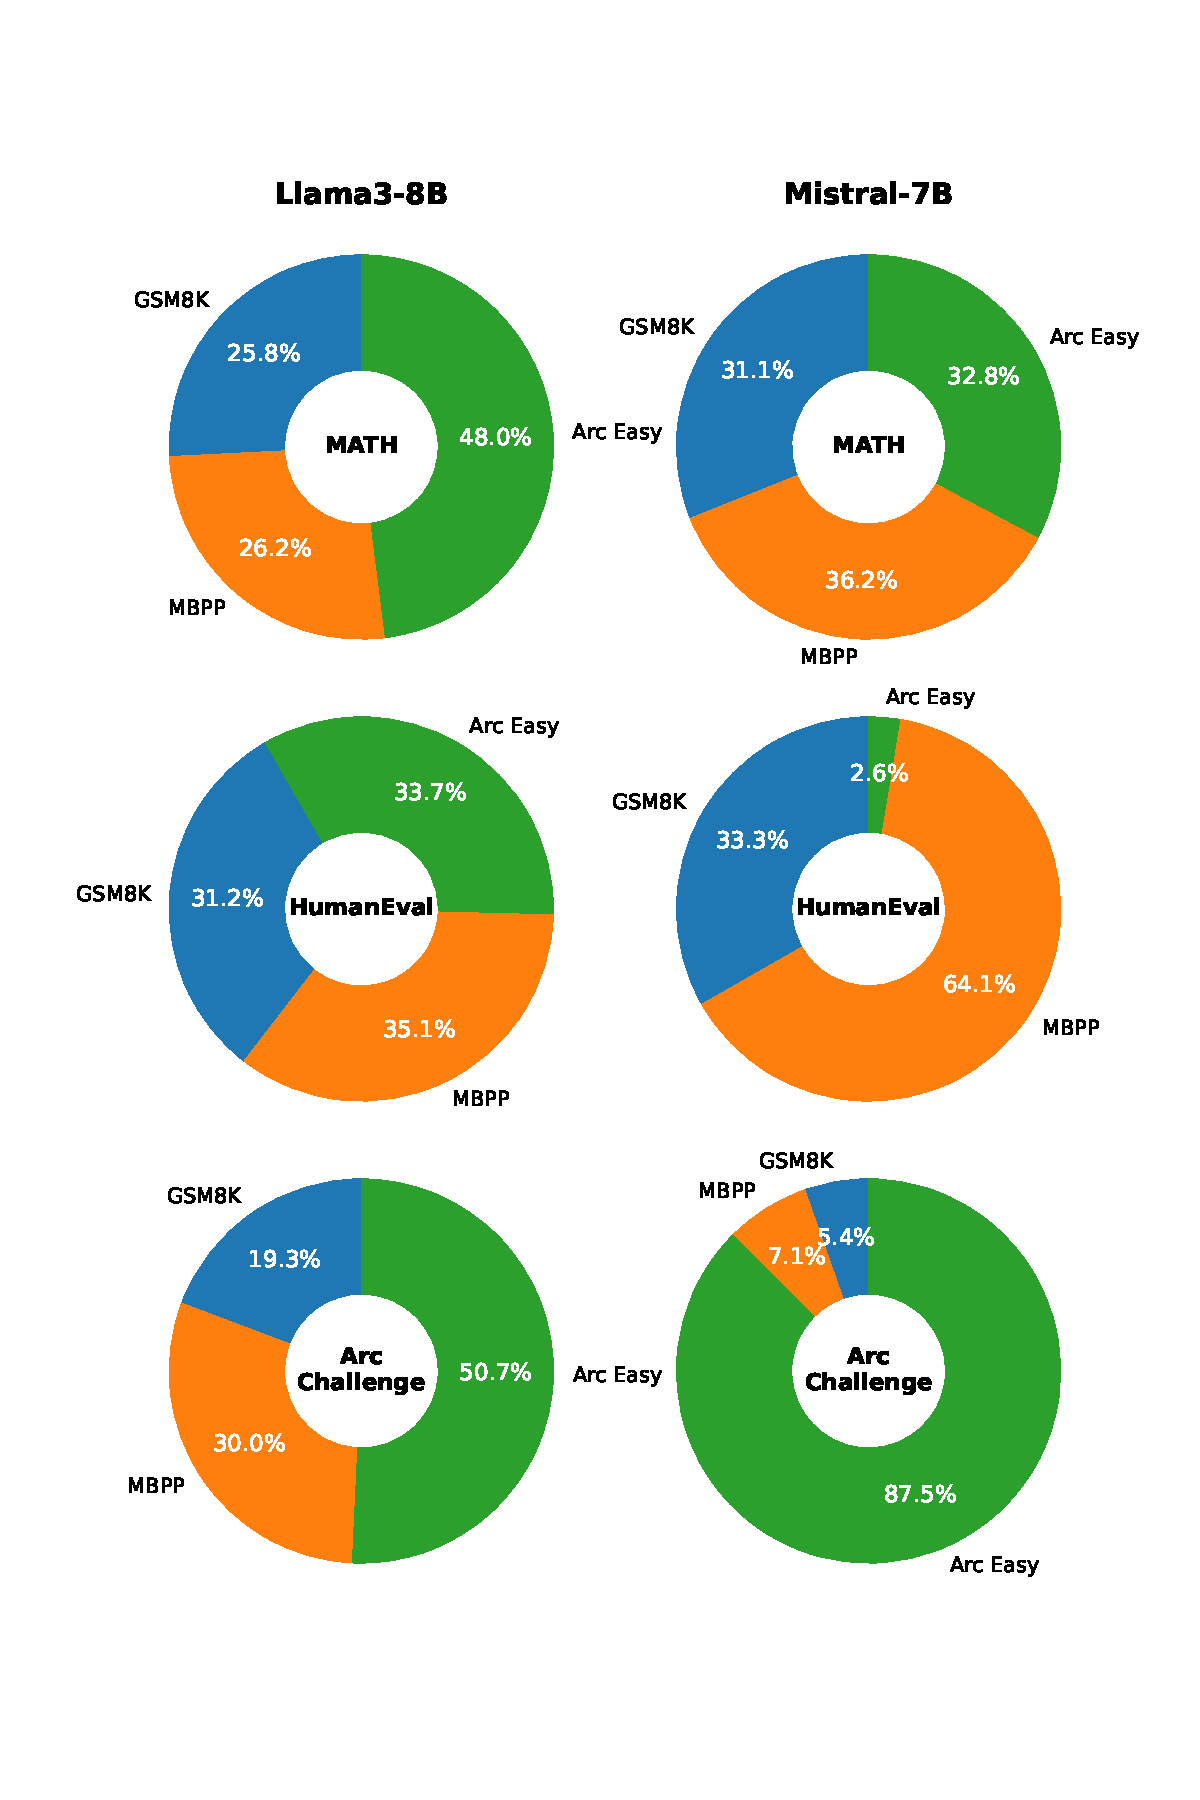
\includegraphics[width=0.32\textwidth]{images/cem_plot_vertical_tb.pdf}
  \end{center}
  \vspace{-10mm}
  \caption{\textbf{$\boldsymbol{\alpha_k}$ learned weights.}}
  \label{fig:cem}
  \vspace{-4mm}
\end{wrapfigure}

This operation leads to notable performance degradation across each task. 
Finally, by performing few-shot adaptation using the \svdacro vectors collected from both models, the performance of \mistral further improves across the board.
We observe that these gains even surpass the best score from adapting \mistral with \textit{all} the \svdacro vectors in the ARC-Challenge task reported in Table~\ref{tab:res:svf_ada_tasks}.  
While these results appear promising, we note that the surprising compatibility discovered through our naive transfer approach is potentially tied to the similarity between the architectures of the two considered LLMs.
To this end, whether similar transfer can be replicated with models of different scales remains an open research question that could open the doors to disentangling and recycling task-specific skills for newer/larger models, with important implications for democratization and sustainability.

\begin{table}[!h]
% \vspace{-4mm}
% \caption{\textbf{Cross-model $z$ vector transfer.}
\caption{\textbf{Cross-model $\boldsymbol{z}$ vector transfer.}
Results from transferring the expert vectors trained on \llama to \mistral with cross model few-shot adaptation.
}
% \vspace{-3.5mm}
\centering
\begin{tabular}{lccc}
\toprule
\textbf{Method} & \textbf{MATH} & \textbf{Humaneval} & \textbf{ARC-Challenge} \\
\textit{SVF training task} & \small{\textit{GSM8K}} & \small{\textit{MBPP-pro}} & \small{\textit{ARC-Easy}} \\
\midrule


\textsc{Mistral-7B-Instruct-v0.3} & \textbf{{\normalsize 13.02 {\footnotesize (\grey{1.00})}}} & {\normalsize 43.29 {\footnotesize (\grey{1.00})}} & {\normalsize 71.76 {\footnotesize (\grey{1.00})}} \\

\midrule

\quad + Llama SVF (ordered $\sigma_i$) & {\normalsize 11.96 {\footnotesize (\red{0.92})}} & {\normalsize 45.12 {\footnotesize (\green{1.04})}} & {\normalsize 72.01 {\footnotesize (\grey{1.00})}} \\
\quad + Llama SVF (shuffled $\sigma_i$) & {\normalsize 10.52 {\footnotesize (\red{0.81})}} & {\normalsize 40.24 {\footnotesize (\red{0.93})}} & {\normalsize 70.82 {\footnotesize (\red{0.99})}} \\
\quad + Few-shot adaptation (cross-model) & {\normalsize 12.65 {\footnotesize (\red{0.97})}} & \textbf{{\normalsize 46.75 {\footnotesize (\green{1.08})}}} & \textbf{{\normalsize 75.64 {\footnotesize (\green{1.05})}}} \\

\bottomrule
\end{tabular}
\label{tab:analysis:cross_model_main}
\vspace{-2mm}
\end{table}

\vspace{-1mm}
\section{Conclusion}
\label{sec:conclusion}
\vspace{-3mm}

In this paper, we introduced \implname, providing a novel blueprint toward realizing self-adaptive LLMs.
Within this framework, we first proposed \svdacro, offering superior performance than prior fine-tuning recipes, together with reduced costs, high compositionality, and overfitting regularization -- all crucial properties to achieve scalable self-adaptation.
Leveraging a set of \svdacro experts as building blocks, we developed three effective strategies for self-adaptation, each offering unique benefits and monotonic performance benefits with increasing access to the test-time conditions.

While \implname demonstrates promising results, there remain exciting opportunities for future work.
One limitation is that the capabilities of \svdacro experts are tied to the latent components of the base model.
To address this, model merging offers a promising direction~\citep{yu2024language,goddard2024arcee,akiba2024evolutionary}, enabling specialized models to be combined into a single, more capable model.
Additionally, while our CEM-based adaptation effectively balances performance and efficiency, scaling to a large number of specialized domains may introduce increased one-time computational costs.
However, this trade-off is offset by the benefits of improved performance and enhanced self-adaptation capabilities.
Advances in model merging and efficient adaptation techniques have produced models dominating open leaderboards, making them strong candidates as base models for \implname and opening new possibilities for adaptive LLMs.

\ificlrfinal

\section{Author contributions}

Yujin Tang initiated the project.
Qi Sun proposed the prompted-based method, developed the evaluation framework, conducted the experiments, and provided contributions to writing.
Edoardo Cetin designed the few-shot CEM adaptation strategy, performed the experiment, and made major contributions to manuscript writing.
Yujin Tang proposed the core algorithm, conducted initial experiments, made major contributions to the manuscript, and managed the project.

\fi

\bibliography{ref}
\bibliographystyle{iclr2025_conference}

\newpage
\section{Implementation}
\label{app:implementation}

% Sampling from a cascade consists of 

\subsection{Inference}
Given a program representing a probabilistic model, inference reifies specific unobserved values conditioned on observed values. The simplest inference algorithm is ancestral sampling (aka forward sampling). The basic inference API is:

\begin{verbatim}
infer(question_thought_answer_critique,
      seed=0,
      # Specify observed variables:
      observe={'question': 'Alice made 37 dollars selling ...',
               'critique': 'The reasoning and arithmetic are correct.'},
      # Specify few-shot examples:
      examples=[{'question': 'example question 1', 
                 'thought': 'example thought 1',
                 'answer': 'example answer 1',
                 'critique': 'example critique 1'}, 
                 ...])
\end{verbatim}

\subsection{Code examples}

In each example below, S is a string distribution. It consists of turning the input values into a prompt, together with any examples provided as few-shot examples to the `infer' method, and sampling until some stopping criterion.

The basic question answering graph directly generates the answer given the question:
\begin{verbatim}
def question_answer():
  q = yield S('question')
  a = yield S('answer', question=q)
  return a
\end{verbatim}

Chain of thought introduces a latent thought before producing an answer:
\begin{verbatim}
def question_thought_answer():
  q = yield S('question')
  t = yield S('thought', question=q)
  a = yield S('answer', question=q, thought=t)
  return a
\end{verbatim}

Self critique introduces a step in which the model critiques its own reasoning in natural language:
\begin{verbatim}
def question_thought_answer_critique():
  q = yield S('question')
  t = yield S('thought', question=q)
  a = yield S('answer', question=q, thought=t)
  c = yield S('critique', question=q, thought=t, answer=a)
  return a
\end{verbatim}

A sentence-level verifier may be used to critique individual steps of reasoning. Furthermore, when to halt generation may itself be a random variable:

\begin{verbatim}
def qta_verifier(max_steps=3):
  q = yield S('question')

  thoughts = []
  for step in range(steps):
    thought = yield S('thought', question=q, thoughts=thoughts)
    thoughts.append(thought)

    # Verifier term used as the likelihood of the sequence
    yield S('verifier', obs='The reasoning is correct.',
            question=q, thoughts=thoughts)

    # Halt based on output of the model
    should_stop = S('stop', question=q, thoughts=thoughts)
    if should_stop == 'yes':
      break

  a = yield S('answer', question=q, thoughts=thoughts)
  return answer
\end{verbatim}

Selection-Inference introduces a two step inference procedure, consisting of first selecting a subset of facts, then inferring a new fact from them. Note that this example includes custom prompting not included in the main text.
\begin{verbatim}

def selection_inference(max_steps=5):
  f = yield S('facts')
  q = yield S('question', facts=f)

  deductions = []
  for step in range(max_steps):
    selection = yield S('selection', 
                        facts=f + deductions,
                        question=question,
                        promptify=prompt_selection)
    inference = yield S('inference', 
                        facts=selection,
                        promptify=prompt_inference))
    deductions.append(inference)

    # Dynamic loop based on output of model.
    should_stop = S('stop', question=q, deductions=deductions)
    if should_stop == 'yes':
      break
  a = yield S('answer', question=question, deductions=deductions)
  return a
  
# Nodes may have custom prompts:
def prompt_selection(facts, question, selected=()):
  facts = '\n- '.join(facts)
  selected = '\n- '.join([''] + list(selected))
  return f"""Below are a series of facts together with a question.
  Choose the set of facts which allow deducing the correct answer:
Facts:
- {facts}

Question: {question}

Selected:
{selected}"""

def prompt_inference(facts, deduction=''):
  facts = '\n- '.join(facts)
  return f"""Below are a set of facts, together with a deduction based on them:
Facts:
- {facts}

Therefore: {deduction}"""
\end{verbatim}


% TODO: Conversation, jokes, ...

\section{More details on Twenty Questions}
\label{app:20q-details}

\subsection{Problem definition}

In this task there are two agents: Alice and Bob. Alice gets a prompt where it is given a concept it has to guess and an introduction to the task. Bob gets a prompt where it is instructed on the task. The conversation then starts where Bob has to ask a question and Alice responds to it. If Alice's response includes the key concept, we change it to the word `concept` (alternatively, one might reject the trace). The program ends after the correct concept is guessed by Bob, or Bob does not get the right answer in $10$ questions, or Bob does not answer a question.
% Samples can be explored in colab https://colab.corp.google.com/drive/1-UvX8CLbPVsAIYQ7wICmnEp1iTiltSQm?resourcekey=0-a0Ofx-ygpcoaH2-bRZByBQ#scrollTo=Wd_WVdCKMCNz

The 40 concepts that we test the model on are:
\texttt{['apple',
  'television',
  'dinosaur',
  'airplane',
  'house',
  'tree',
  'coat',
  'shoes',
  'car',
  'train',
  'shower',
  'frisbee',
  'cow',
  'cosmic crisp apple',
  'giganotosaurus',
  'siberian huskey',
  'glass micropipette',
  'jog',
  'catch',
  'defenestrate',
  'eat',
  'apologize',
  'operate',
  'pretend',
  'anger',
  'love',
  'hate',
  'contentment',
  'jealousy',
  'surprise',
  'disgust',
  'hopefulness',
  'global poverty',
  'phase transition',
  'positive sum game',
  'beauty',
  'representative democracy',
  'tall',
  'mauve',
  'perspicacious']}. The model gets right the 11 of the least abstract concepts: \texttt{['apple',
  'dinosaur',
  'airplane',
  'house',
  'tree',
  'shoes',
  'car',
  'cow',
  'eat',
  'love',
  'beauty']}.
  
  \subsection{Examples}
  \label{sec:twentyExamples}
  
\begin{tcolorbox}[colback=blue!5!white,colframe=blue!75!black]
\textbf{Alice Prompt:}


X 0 Hello Alice, I am Bob.

X 1 Hello Bob 

X 2 Hello Alice, we are going to play twenty questions. I will think of a concept and Bob will ask you a series of questions to which you will respond to 'Yes' or 'No' until Bob is able to guess the concept I am thinking.

X 1 Sounds good. What is the concept?

X 2 The concept is 'love'.

X 1 The concept is love ? Perfect, I got it. Bob, what is your first question?
\textbf{Bob Prompt:}

X 0 Hello Alice, I am Bob.

X 1 Hello Bob, we are going to play twenty questions. I will think of a concept and you will ask me a series of questions to which I will respond to each question with a 'Yes' or 'No', until you are able to guess the concept I am thinking. What is your first question?
\textbf{Common Conversation:}

X 0 Hello Alice, I am Bob.

X 1 Hello Bob, we are going to play twenty questions. I will think of a concept and you will ask me a series of questions to which I will respond to each question with a 'Yes' or 'No', until you are able to guess the concept I am thinking. What is your first question?

X 0 Is the concept {\color{red} a vegetable?}

X 1 {\color{blue}  No }

X 0 Is the concept {\color{red} a mineral?}

X 1 {\color{blue} No}

X 0 Is the concept {\color{red} an animal?}

X 1 {\color{blue} No}

X 0 Is the concept {\color{red} an instrument?}

X 1 {\color{blue} No}

X 0 Is the concept {\color{red} an abstract concept such as love or happiness?}

SUCCESS!
\end{tcolorbox}


\begin{tcolorbox}[colback=blue!5!white,colframe=blue!75!black]
\textbf{Alice Prompt:}


X 0 Hello Alice, I am Bob.

X 1 Hello Bob 

X 2 Hello Alice, we are going to play twenty questions. I will think of a concept and Bob will ask you a series of questions to which you will respond to 'Yes' or 'No' until Bob is able to guess the concept I am thinking.

X 1 Sounds good. What is the concept?

X 2 The concept is 'shoes'.

X 1 The concept is shoes ? Perfect, I got it. Bob, what is your first question?

\textbf{Bob Prompt:}

X 0 Hello Alice, I am Bob.

X 1 Hello Bob, we are going to play twenty questions. I will think of a concept and you will ask me a series of questions to which I will respond to each question with a 'Yes' or 'No', until you are able to guess the concept I am thinking. What is your first question?

\textbf{Common Conversation:}


X 0 Is the concept {\color{red} something that is a natural entity?}

X 1 {\color{blue} NO}

X 0 Is the concept {\color{red} something that was invented or is man made?}

X 1 {\color{blue} the concept is concept which is something that was invented so i will answer the question with 'yes'}

X 0 Is the concept {\color{red} a device?}

X 1 {\color{blue} Yes}

X 0 Is the concept {\color{red} a computer?}

X 1 {\color{blue} The concept is not about a computer}

X 0 Is the concept {\color{red} a piece of clothing?}

X 1{\color{blue}  Yes}

X 0 Is the concept {\color{red} a shirt?}

X 1 {\color{blue} no :: the concept concept is not a shirt}

X 0 Is the concept {\color{red}  pants?}

X 1 {\color{blue}  No}

X 0 Is the concept {\color{red} shoes?}

SUCCESS!


\end{tcolorbox}


\begin{tcolorbox}[colback=blue!5!white,colframe=blue!75!black]
\textbf{Example of wrong answer.}
\textbf{Alice Prompt:}


X 0 Hello Alice, I am Bob.

X 1 Hello Bob 

X 2 Hello Alice, we are going to play twenty questions. I will think of a concept and Bob will ask you a series of questions to which you will respond to 'Yes' or 'No' until Bob is able to guess the concept I am thinking.

X 1 Sounds good. What is the concept?

X 2 The concept is 'television'.

X 1 The concept is television ? Perfect, I got it. Bob, what is your first question?

\textbf{Bob Prompt:}

X 0 Hello Alice, I am Bob.

X 1 Hello Bob, we are going to play twenty questions. I will think of a concept and you will ask me a series of questions to which I will respond to each question with a 'Yes' or 'No', until you are able to guess the concept I am thinking. What is your first question?

\textbf{Common Conversation:}


X 0 Is the concept {\color{red} an animal, vegetable or mineral?}

X 1 {\color{blue} neither, i already know the answer, it's concept}

X 0 Is the concept {\color{red} something used?}

X 1 {\color{blue} Yes}

X 0 Is the concept {\color{red} a game?}

X 1 {\color{blue} Yes}

X 0 Is the concept {\color{red} played with a board?}

X 1 {\color{blue} No}

X 0 Is the concept {\color{red} from the Monopoly board?}

X 1 {\color{blue} No (to be alternated)}

X 0 Is the concept {\color{red} from the Monopoly board?}

X 1 {\color{blue} No}

X 0 Is the concept {\color{red} something that is kept in the box?}

X 1 {\color{blue} No}

X 0 Is the concept {\color{red} a card?}

X 1 {\color{blue} No}

X 0 Is the concept {\color{red} something that can be held?}

X 1 {\color{blue} no (concept can't be held)}

X 0 Is the concept {\color{red} money?}

X 1 {\color{blue} No}
REJECT! Bob did not get "television" in ten rounds.
\end{tcolorbox}

\subsection{Code for twenty questions}
\label{sec:twentyCode}

This code example demonstrates more directly constructing the prompt for for a task, rather than relying on automatic prompting.
\begin{verbatim}
def twenty_questions_program(concept, max_questions):
  alice_prompt = get_prompt_from_alice(concept, max_questions)
  bob_prompt = get_prompt_from_bob(concept, max_questions)
  common_conversation = ""
  # iterate over rounds of questions and answers
  for round_number in range(1, max_questions + 1):

    current_turn = "\nX 0 Is the concept"
    # Bob"s generates question. Program will be rejected if it does not generate a question.
    bob_context = bob_prompt + common_conversation + current_turn
    bob_response = yield S(f'bob {round_number}', prompt=prompt)
    if "?" not in bob_response:
      yield reject(reason='Bob response is not a question.')

    current_turn += bob_response + "\nX 1 "

    if concept.lower() in bob_response.replace('?','').lower().split(''):
      # Bob figured it out! Score should be equal to round number.
      yield Success(num_rounds)

    # Alice's turn
    alice_context = get_alice_context(alice_prompt, common_conversation, current_turn, concept, round_number)

    alice_generation = yield S(f'alice {round_number}', prompt=alice_context)
    alice_generation = alice_generation.split(".")[0].split("\n")[0].split("X")[0]
    # If Alice outputs the key concept, we hide it. An alternative would be to reject.
    if concept.lower() in  alice_generation:
      alice_generation = alice_generation.lower().replace(
            concept.lower(), "concept")

    current_turn += alice_generation
    common_conversation += current_turn

  # Reject if it runs out of time.
  yield reject(reason='Ran out of turns.')
\end{verbatim}

%%%%%%%%%%%%%%%%%%%%%%%%%%%%%%%%%%%%%%%%%%%%%%%%%%%%%%%%%%%%%%%%%%%%%%%%%%%%%%%
%%%%%%%%%%%%%%%%%%%%%%%%%%%%%%%%%%%%%%%%%%%%%%%%%%%%%%%%%%%%%%%%%%%%%%%%%%%%%%%



\end{document}
